% Options for packages loaded elsewhere
\PassOptionsToPackage{unicode}{hyperref}
\PassOptionsToPackage{hyphens}{url}
\PassOptionsToPackage{dvipsnames,svgnames,x11names}{xcolor}
%
\documentclass[
  number]{elsarticle}

\usepackage{amsmath,amssymb}
\usepackage{iftex}
\ifPDFTeX
  \usepackage[T1]{fontenc}
  \usepackage[utf8]{inputenc}
  \usepackage{textcomp} % provide euro and other symbols
\else % if luatex or xetex
  \usepackage{unicode-math}
  \defaultfontfeatures{Scale=MatchLowercase}
  \defaultfontfeatures[\rmfamily]{Ligatures=TeX,Scale=1}
\fi
\usepackage{lmodern}
\ifPDFTeX\else  
    % xetex/luatex font selection
\fi
% Use upquote if available, for straight quotes in verbatim environments
\IfFileExists{upquote.sty}{\usepackage{upquote}}{}
\IfFileExists{microtype.sty}{% use microtype if available
  \usepackage[]{microtype}
  \UseMicrotypeSet[protrusion]{basicmath} % disable protrusion for tt fonts
}{}
\makeatletter
\@ifundefined{KOMAClassName}{% if non-KOMA class
  \IfFileExists{parskip.sty}{%
    \usepackage{parskip}
  }{% else
    \setlength{\parindent}{0pt}
    \setlength{\parskip}{6pt plus 2pt minus 1pt}}
}{% if KOMA class
  \KOMAoptions{parskip=half}}
\makeatother
\usepackage{xcolor}
\setlength{\emergencystretch}{3em} % prevent overfull lines
\setcounter{secnumdepth}{5}
% Make \paragraph and \subparagraph free-standing
\ifx\paragraph\undefined\else
  \let\oldparagraph\paragraph
  \renewcommand{\paragraph}[1]{\oldparagraph{#1}\mbox{}}
\fi
\ifx\subparagraph\undefined\else
  \let\oldsubparagraph\subparagraph
  \renewcommand{\subparagraph}[1]{\oldsubparagraph{#1}\mbox{}}
\fi


\providecommand{\tightlist}{%
  \setlength{\itemsep}{0pt}\setlength{\parskip}{0pt}}\usepackage{longtable,booktabs,array}
\usepackage{calc} % for calculating minipage widths
% Correct order of tables after \paragraph or \subparagraph
\usepackage{etoolbox}
\makeatletter
\patchcmd\longtable{\par}{\if@noskipsec\mbox{}\fi\par}{}{}
\makeatother
% Allow footnotes in longtable head/foot
\IfFileExists{footnotehyper.sty}{\usepackage{footnotehyper}}{\usepackage{footnote}}
\makesavenoteenv{longtable}
\usepackage{graphicx}
\makeatletter
\def\maxwidth{\ifdim\Gin@nat@width>\linewidth\linewidth\else\Gin@nat@width\fi}
\def\maxheight{\ifdim\Gin@nat@height>\textheight\textheight\else\Gin@nat@height\fi}
\makeatother
% Scale images if necessary, so that they will not overflow the page
% margins by default, and it is still possible to overwrite the defaults
% using explicit options in \includegraphics[width, height, ...]{}
\setkeys{Gin}{width=\maxwidth,height=\maxheight,keepaspectratio}
% Set default figure placement to htbp
\makeatletter
\def\fps@figure{htbp}
\makeatother

\usepackage{booktabs}
\usepackage{caption}
\usepackage{longtable}
\makeatletter
\@ifpackageloaded{float}{}{\usepackage{float}}
\floatstyle{plain}
\@ifundefined{c@chapter}{\newfloat{suppplot}{h}{losuppplot}}{\newfloat{suppplot}{h}{losuppplot}[chapter]}
\floatname{suppplot}{Figure S}
\newcommand*\quartosuppplotref[1]{Figure \hyperref[#1]{S\ref{#1}}}
\@ifpackageloaded{caption}{}{\usepackage{caption}}
\DeclareCaptionLabelFormat{quartosuppplotreflabelformat}{#1#2}
\captionsetup[suppplot]{labelformat=quartosuppplotreflabelformat}
\newcommand*\listofsuppplots{\listof{suppplot}{List of Supplementary Figures}}
\makeatother
\makeatletter
\@ifpackageloaded{float}{}{\usepackage{float}}
\floatstyle{plain}
\@ifundefined{c@chapter}{\newfloat{supptab}{h}{losupptab}}{\newfloat{supptab}{h}{losupptab}[chapter]}
\floatname{supptab}{Table S}
\newcommand*\quartosupptabref[1]{Table \hyperref[#1]{S\ref{#1}}}
\@ifpackageloaded{caption}{}{\usepackage{caption}}
\DeclareCaptionLabelFormat{quartosupptabreflabelformat}{#1#2}
\captionsetup[supptab]{labelformat=quartosupptabreflabelformat}
\newcommand*\listofsupptabs{\listof{supptab}{List of Supplementary Tables}}
\makeatother
\makeatletter
\@ifpackageloaded{caption}{}{\usepackage{caption}}
\AtBeginDocument{%
\ifdefined\contentsname
  \renewcommand*\contentsname{Table of contents}
\else
  \newcommand\contentsname{Table of contents}
\fi
\ifdefined\listfigurename
  \renewcommand*\listfigurename{List of Figures}
\else
  \newcommand\listfigurename{List of Figures}
\fi
\ifdefined\listtablename
  \renewcommand*\listtablename{List of Tables}
\else
  \newcommand\listtablename{List of Tables}
\fi
\ifdefined\figurename
  \renewcommand*\figurename{Figure}
\else
  \newcommand\figurename{Figure}
\fi
\ifdefined\tablename
  \renewcommand*\tablename{Table}
\else
  \newcommand\tablename{Table}
\fi
}
\@ifpackageloaded{float}{}{\usepackage{float}}
\floatstyle{ruled}
\@ifundefined{c@chapter}{\newfloat{codelisting}{h}{lop}}{\newfloat{codelisting}{h}{lop}[chapter]}
\floatname{codelisting}{Listing}
\newcommand*\listoflistings{\listof{codelisting}{List of Listings}}
\makeatother
\makeatletter
\makeatother
\makeatletter
\@ifpackageloaded{caption}{}{\usepackage{caption}}
\@ifpackageloaded{subcaption}{}{\usepackage{subcaption}}
\makeatother
\ifLuaTeX
  \usepackage{selnolig}  % disable illegal ligatures
\fi
\usepackage[]{natbib}
\bibliographystyle{elsarticle-num}
\usepackage{bookmark}

\IfFileExists{xurl.sty}{\usepackage{xurl}}{} % add URL line breaks if available
\urlstyle{same} % disable monospaced font for URLs
\hypersetup{
  pdftitle={Effect of Sampling Design on Characterizing Surface Soil Fingerprinting Properties},
  pdfauthor={Maria Alejandra Luna Miño; Alexander J Koiter; David A Lobb},
  pdfkeywords={Sediment fingerprinting, Sampling design, Soil
characterization},
  colorlinks=true,
  linkcolor={blue},
  filecolor={Maroon},
  citecolor={Blue},
  urlcolor={Blue},
  pdfcreator={LaTeX via pandoc}}

\setlength{\parindent}{6pt}
\begin{document}

\begin{frontmatter}
\title{Effect of Sampling Design on Characterizing Surface Soil
Fingerprinting Properties}
\author[1]{Maria Alejandra Luna Miño%
%
}
 \ead{steve@curvenote.com} 
\author[2]{Alexander J Koiter%
\corref{cor1}%
}
 \ead{koitera@brandonu.ca} 
\author[3]{David A Lobb%
%
}
 \ead{David.Lobb@umanitoba.ca} 

\affiliation[1]{organization={Brandon University, Masters in
Environmental and Life Sciences},addressline={270 18th
St},city={Brandon},postcode={R7A 6A9},postcodesep={}}
\affiliation[2]{organization={Brandon University, Department of
Geography and Environment},addressline={270 18th
St},city={Brandon},postcode={R7A 6A9},postcodesep={}}
\affiliation[3]{organization={University of Manitoba, Department of of
Soil Science},addressline={13 Freedman
Crescent},city={Winnipeg},postcode={R3T 2N2},postcodesep={}}

\cortext[cor1]{Corresponding author}



        
\begin{abstract}
Purpose: The characterization of soil properties is an important part of
many different types of agri-environmental research including inventory,
comparison, and manipulation studies. Sediment source fingerprinting is
a method that is increasingly being used to link sediment sources to
downstream sediment. There is currently not a standard approach to
characterizing sources and the different approaches to sampling have not
been well assessed. Methods: Grid (n=49), transect (n=14), and likely to
erode (n=8) sampling designs were used to characterize the geochemical,
colour, grain size distribution, and soil organic matter content at two
sites under contrasting land uses (agricultural and forested). The
impact of the three sampling designs on characterization of fingerprint
properties, the relationship between particle size and organic matter
content on fingerprint properties, fingerprint selection, source
discrimination, and mixing apportionment results were evaluated using a
range of methods including 21 virtual mixtures. Results: The likely to
erode design resulted in a unique fingerprint signature compared to the
other two sampling designs. The correlation between particle size and
organic matter on fingerprint properties varied between fingerprint,
source, and sampling design. While the number and composition of the
fingerprints selected varied between sampling designs there was strong
(100\%) discrimination between sources regardless of the sampling
approach. The maximum absolute difference between the virtual mixtures
and the modeled proportions was 7.65, 7.80, and 8.93\% for the grid,
transect, and likely to erode sampling designs, respectively.
Conclusions: The likely to erode sampling design was not representative
of the upslope areas as characterized by the grid and transect methods.
Despite these differences the final apportionment results using virtual
mixtures were qualitatively similar between the three sampling designs.
Continued work at the watershed scale is needed to fully evaluate the
importance of source sampling design on the sediment source
fingerprinting approach.
\end{abstract}





\begin{keyword}
    Sediment fingerprinting \sep Sampling design \sep 
    Soil characterization
\end{keyword}
\end{frontmatter}
    
\section{Introduction}\label{introduction}

\subsection{Sediment pollution and
erosion}\label{sediment-pollution-and-erosion}

Sediment pollution has been identified as a major cause of surface water
impairment, and sediment is considered to be a common pollutant in many
watersheds \citep{owens2005}. Agriculture was found to be a key threat
to water quality because of high sediment and nutrient loads
\citep{vörösmarty2010}. Excessive sediment loads can have negative
impacts on biota healthiness, result in eutrophication, and increase the
cost of preserving drainage ditches. Suitable management practices can
be implemented across watersheds to reduce sediment load and erosion in
different land uses \citep{noe2020}. Moreover, fine sediment represents
a substantial diffuse source pollutant in surface water because of its
role in governing the transfer and fate of nutrients, heavy metals,
pesticides and due to its impacts on aquatic ecology
\citep{walling2008}. Sediment delivered to streams has been considered a
main source of impairment of streams and watersheds \citep{bilotta2008}.
Therefore, semi-empirical information to identify the origins of
sediment sources can be used to target management strategies
\citep{mukundan2012}. Sediment fingerprinting links sources to
downstream sediment using natural fingerprints (e.g., physical or
biogeochemical properties) and uses an unmixing model to estimate the
contributions from each source. For an overview and examples of
methodology and applications see \citep{collins1997},
\citep{walling2008}, \citep{davis2009}, \citep{owens2016},
\citep{collins2020}, and \citep{evrard2022}.

\subsection{Potential source
characterization}\label{potential-source-characterization}

Characterizing potential sources of sediment may be a problematic and
complicated task yet is an important step in the sediment fingerprinting
technique. This step may be difficult to accomplish since the different
approaches reported in the literature have not been well evaluated, and
there is not a standard approach to characterize sources
\citep{collins2020}. There is a broad range in source and in-stream
sediment sampling designs used \citep[e.g.,][]{boudreault2019}. These
approaches have included the sampling of areas likely to be eroded, but
not necessarily actively eroding \citep{collins1997}, a targeted
sampling of actively eroding sites \citep{wallbrink2004} and
transect/grid sampling \citep{miller2005}. The characterization of the
potential sources typically has three main goals: 1) assess the impact
of grain size and organic matter content on fingerprint properties, 2)
identify fingerprinting properties that have the ability to discriminate
between sources, and 3) serve as end members for the unmixing model.
While each of these have been previously investigated, the focus has
been more on implications of how the data is processed post sampling
\citep[e.g.,][]{haddadchi2014, smith2014, laceby2015, laceby2017, batista2022}.

Along the sediment cascade from source to downstream sediment there is
typically a degree of sorting resulting in a shift in both particle size
distribution and organic matter content. Given the strong dependency of
many fingerprints on these two properties, steps are typically taken
into account for the shift in grain size. This is typically done through
a combination of sieving to remove coarse-grained material and further
application of additional corrections (e.g., normalization, regression)
\citep{laceby2017}. The latter step requires information on both the
grain size and organic matter content in addition to fingerprint
composition where the nature and quality of the data is dependent on the
sampling design used. Similarly, the sampling design used to
characterize the mean and variability of fingerprint properties will
influence which fingerprints provide the best discrimination between
sources. Most selection methods preferentially select fingerprints that
have low within source variability and large differences between sources
\citep{pulley2017}. Together, these two steps provide the end members
used in mixing models and the final apportionment results will be a
reflection of the quality of these inputs.

The lack of standardization in sampling designs makes it difficult to
compare results between studies as the differences in sampling designs
represent an unquantified source uncertainly
\citep[e.g.,][]{koiter2013}. An effective sampling campaign is designed
to efficiently collect samples that are representative of the potential
sources of sediment identified within a watershed. The importance of the
sampling campaign variables, including the number of samples collected,
sampling methods, and sampling design developed to characterize sources
is not well understood and it may influence the final sediment
fingerprinting apportionment results \citep{collins2020}. Source
sampling typically occurs at two scales of observation. The watershed
scale captures the variability within the sources across different
regions or physiographic units. The local scale sampling (e.g.,
individual fields or streambanks within a reach) is where the
variability across a catena or along the depth of streambank is captured
\citep{collins2020}. The focus of this paper is on sampling at the local
scale, but it is important to note that sampling at the watershed scale
is of equal importance.

Using expert knowledge, the likely to erode approach identifies sources
with a high probability to contribute sediment to streams. An advantage
of this approach is that it allows for the selection of sampling areas
close to drainage pathways which are conceptually and physically more
directly linked to the downstream sediment. The disadvantage is that the
sampling choices made will vary between individuals/experts and it
provides no information on soil properties and processes further up
slope (i.e., limited context). In contrast, a randomized sampling
approach overcomes the issues of the expert-based opinion in the likely
to erode approach, one of the limitations is potentially missing
important landscape features resulting in an inadequate
characterization. This limitation can be partially offset by a
stratified random sampling approach whereby distinctive units are first
identified and sampling is randomized within each predefined unit
\citep{pennock2008}.

A commonly used sampling design for various field studies is systematic
sampling using either transects \citep[e.g.,][]{du2017} or grids
\citep[e.g.,][]{lauzon2005}. The transect is used for a variety of field
studies to show the changes of soil properties along a toposequence
parallel to the dominant slope gradient which can extend from the edge
of the streambank to the hilltop. This sampling design is recommended to
understand the variation of soil properties along the catena as the
variability in this direction is typically the largest and the most
informative \citep{pennock2008}. In terms of determining the spacing of
samples, soil samples can be collected from equally spaced locations,
based on hill slope position, or other landscape features (e.g., edge of
field, fence lines).

The grid sampling design is often used for spatial pattern studies
because of the ease with which pattern maps can be derived from the
grids. Grid sampling designs tend to be a more expensive method employed
in soil sampling because of the large number of samples that need to be
collected, processed, and analyzed. However, they can provide highly
detailed information about the distribution of variability in soil
properties \citep{pennock2008}. Geostatistical approaches typically use
grid sampling designs \citep{pennock2008}. For example, Cambardella et
al. \citep{cambardella1994} demonstrated that grid sampling designs
allows for field-scale variability in soil properties to be assessed
beyond univariate statistics (e.g., mean, standard deviations) and can
provide additional insight into the underlying processes resulting in
the observed patterns. In general, the sampling spacing should be
smaller than the distance between relevant landforms in the field
\citep{pennock2008}. When available, sample spacing can be based on
prior knowledge of the area and may include soil maps, visual
observation of vegetation/yield, or past research studies.

The sediment fingerprinting technique has identified a wide range of
potential sources of sediments, for example: arable lands
\citep[e.g.,][]{russell2001}, pasture lands \citep[e.g.,][]{blake2012},
gully erosion areas \citep[e.g.,][]{evrard2013}, channel banks
\citep[e.g.,][]{collins2010}, landslides \citep[e.g.,][]{nelson2002},
and urban sources \citep[e.g.,][]{carter2003}. The number and nature of
the potential sources of sediment identified will vary among watersheds.
This variation is mostly related to geology, geomorphology, soil type,
hydrology, spatial scale, topography, and land use. The quality of the
representation of potential sources of sediment are largely based on the
sampling design used. The sampling design has multiple and cascading
effects within the fingerprinting framework, including estimates of mean
and variance, fingerprint selection, discrimination potential, and
apportionment results. Therefore, careful consideration needs to be
given to this step to achieve reliable and robust apportionment results.

The three main objectives of this study are to: 1) compare three unique
sampling approaches (transect, grid, and likely to erode) in
characterizing potential sources of sediment; 2) evaluate the impact of
sampling designs on fingerprinting selection and evaluate the ability to
discriminate between a forested and agricultural site; and 3) determine
the implications of different sampling designs on the final
apportionment results using virtual mixtures. Overall, addressing these
objectives will lead to improvement of the sediment fingerprinting
approach and lead to more robust and reliable results.

\section{Material and Methods}\label{material-and-methods}

\subsection{Site descriptions}\label{site-descriptions}

The Wilson Creek watershed (WCW) is located in south-western Manitoba,
Canada near the town of McCreary (Figure~\ref{fig-map}). The WCW
headwaters are on top of the Manitoba Escarpment, and the stream drops
300 metres as it crosses the escarpment. Beyond the escarpment, there is
an alluvial fan, which lies in the lacustrine deposits of glacial Lake
Agassiz \citep{mcginn1979} (Figure~\ref{fig-map}). The upper portion of
the watershed is within the boundaries of Riding Mountain National Park
where the development is restricted to recreational hiking trails and is
forested. Downstream of the park boundary, the land use is agriculture,
and the stream is enclosed in an engineered drainage ditch to the point
where it enters the Turtle River \citep{mackay1970, mcginn1979}.

\begin{figure}

\centering{

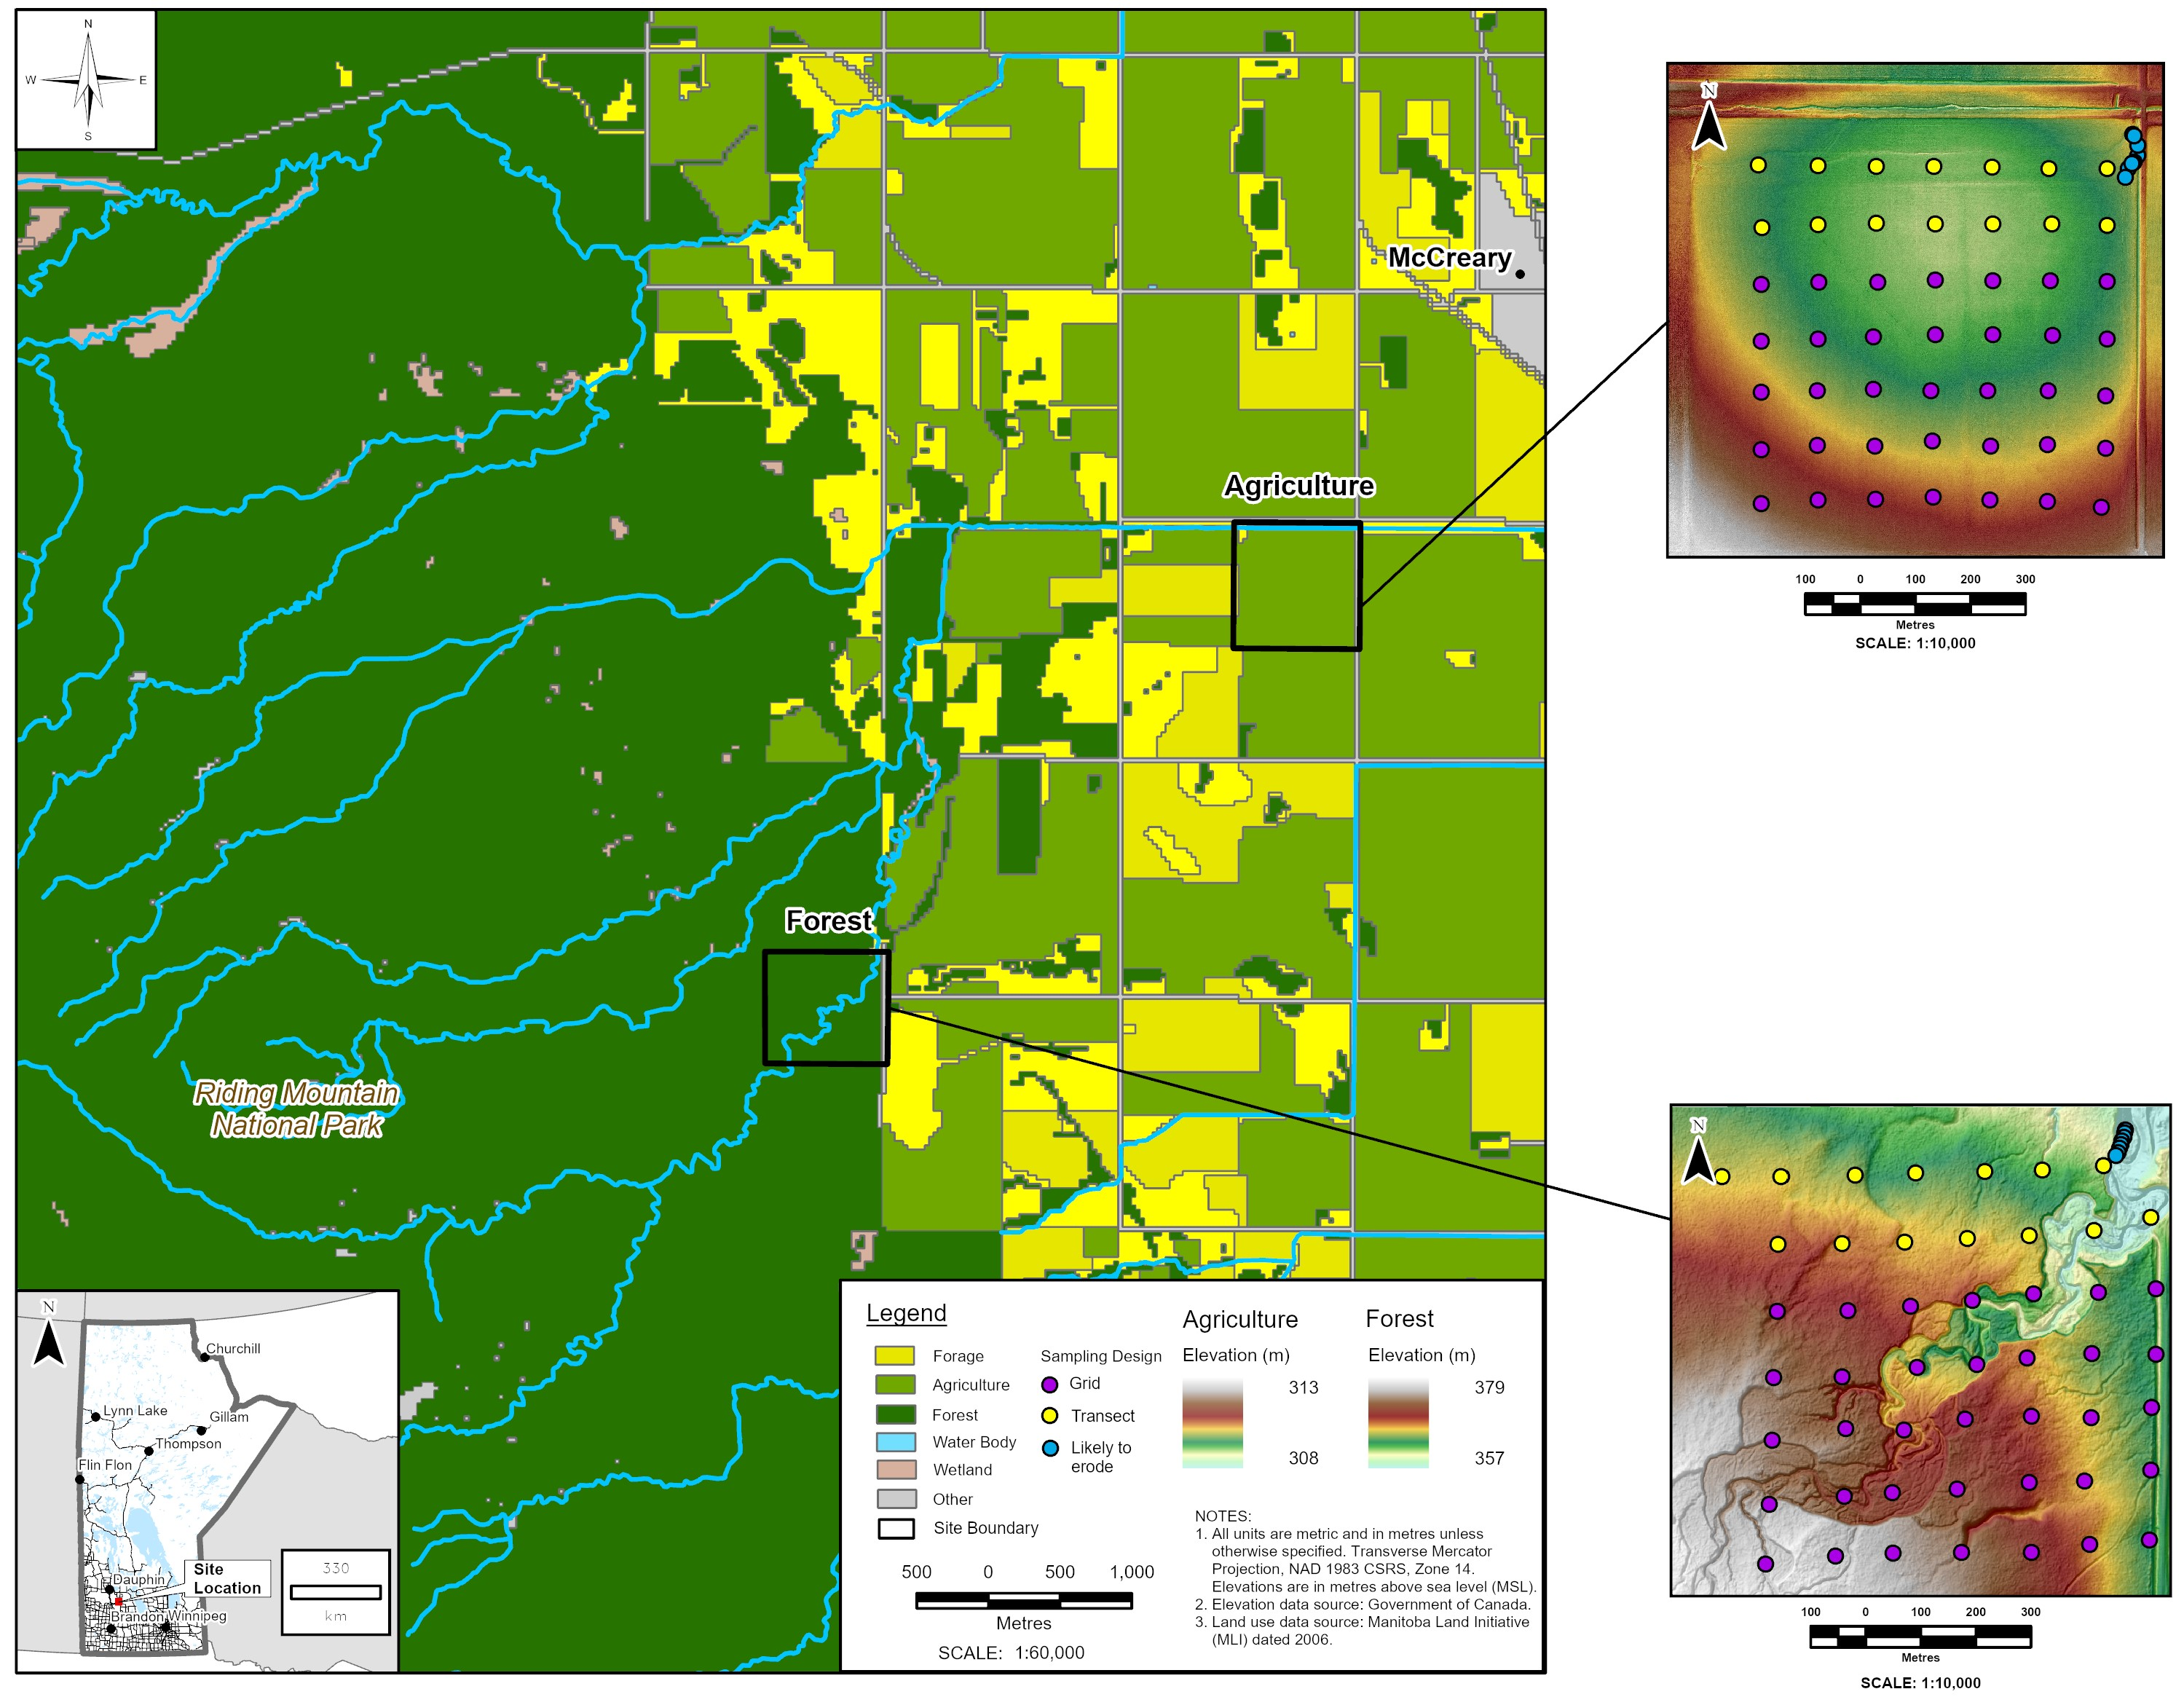
\includegraphics{images/Figure_1.jpg}

}

\caption{\label{fig-map}Location of study sites in south-western
Manitoba, Canada. Regional land use digital elevation model, and
sampling points for the two study sites. Note the transect samples are
also part of the grid sampling design.}

\end{figure}%

The climate of the region is classified as sub-humid with an average
annual precipitation of approximately 538.9 mm, with approximately 27\%
falling as snow. The mean annual temperature is 3.0°C \citep[1981--2010
climate normals,][]{environmentandclimatechangecanada2024}, and the
hydrology of the watershed is characterized as snowmelt dominated with
\textasciitilde{} 80\% of the cumulative runoff occurring during the
spring season (May and June) \citep{mackay1970}. The dominant soils in
the area are Chernozems (Black-Meadow soils) and are developed on thin,
loam to clay loam lacustrine deposits, which lie over reworked boulder
till. Surface soil textures range from fine sandy loam to clay loam
\citep{ehrlich1958}. Visual observations of erosional and depositional
features indicate that forested and agricultural areas in the watershed
are contributing sediment.

he two sites encompassing the predominant land uses within the WCW
(Figure~\ref{fig-map}) and adjacent to the mainstem were selected to
investigate the implications of source sampling designs on commonly used
fingerprinting properties. Both sites are located on an alluvial fan,
where the apex is situated at the base of the escarpment where there is
an abrupt change in gradient and the stream is no longer deeply incised.
The forested site is characterized by a lower gradient stream relative
to the stream crossing over the Manitoba Escarpment, floodplains, and a
meandering channel form \citep{mcginn1979} (Figure~\ref{fig-map}). The
forested site is bounded by the park boundary to the west and the
vegetation is principally mixedwood with including white and black
spruce (Picea glauca, Picea mariana), balsam fir (Abies balsamea), larch
(Larix laricina) and young stands of deciduous trees including trembling
aspen (Populus tremuloides) and white birch (Betula papyrifera). The
agriculture site is low relief and the agricultural production in the
field includes rotations of grain crops and forage. The field is bounded
by the Wilson Creek (engineered channel) on the north and a secondary
surface drain on the east and other fields on the south and west
(Figure~\ref{fig-map}) \citep{mcginn1979}.

\subsection{Sampling design}\label{sampling-design}

Transect, grid, and likely to erode sampling designs were used to
characterize the fingerprint properties of both the agricultural and
forested sites (Figure~\ref{fig-map}). Across all three different
sampling designs, a total of 114 unique sampling points were established
with 57 samples collected at both sites. At each of the sampling points,
a soil auger was used to sample surface soil from 0-15 cm (to account
for depth of regular tillage) in the agricultural field and from 0-5 cm
below the LFH layer in the forested site.

The transect sampling design consisted of two parallel transects with 7
sampling points per transect, spaced at a distance of 100 m apart. The
two transects were orientated parallel to the predominant drainage
pathway for the agricultural site and perpendicular to the stream for
the forested site. For the grid sampling design, an additional 35
samples per site spaced at 100 m were collected creating a 7x7 grid. At
the forested site eight likely to eroded source samples were collected
on the flood plain parallel to the stream at the north-east corner of
the 7x7 grid. At the agricultural site eight likely to erode source
samples were collected at the field edge where infield drainage pathways
directly connected the field to the secondary surface drain.

\subsection{Laboratory analysis}\label{laboratory-analysis}

Source samples were air-dried, manually disaggregated using a mortar and
pestle and passed through a 2-mm stainless steel sieve to remove coarse
fragments and vegetation and a subsample was further sieved to
\textless{} 63 µm. Previous work has shown that sieving to \textless{}
63 µm is an effective way to reduce the differences in particle size and
organic matter between different sources \citep{laceby2017}. For
particle size analysis, samples were digested with hydrogen peroxide
(35\%) to remove organic matter and an aliquot of a dispersing agent of
sodium hexametaphosphate was added following the procedure of Kroetsch
and Cang \citep{kroetsch2007}. The grain size distribution and specific
surface area (SSA) was measured using a Mastersizer 3000, laser
diffraction system (Malvern, UK; 0.01 -- 3500 μm diameter measurement
range). A constant particle density of 2.65 g cm-3 was used to estimate
the SSA. Soil organic matter (SOM) content was determined using
loss-on-ignition. Following the procedure of Nelson and Sommers
\citep{nelson1996}, three grams of oven-dried soil (105°C for 24 hours)
were ashed at 400°C for 16 hours. Organic matter and grain size were
analyzed as supporting information to help interpret the observed
variability in surface soil fingerprint properties.

All soil samples were analyzed through a commercial laboratory (ALS
Mineral Division, North Vancouver, BC, Canada) for a broad suite of 51
geochemical elements (Ag, Al, As, Au, B, Ba, Be, Bi, Ca, Cd, Ce, Co, Cr,
Cs, Cu, Fe, Ga, Ge, Hf, Hg, In, K, La, Li, Mg, Mn, Mo, Na, Nb, Ni, P,
Pb, Rb, Re, S, Sb, Sc, Se, Sn, Sr, Ta, Te, Th, Ti, Tl, U, V, W, Y, Zn
and Zr) using inductively coupled plasma mass spectrometry (ICP-MS)
following a microwave-assisted digestion with aqua-regia. However, of
the 51 geochemical elements examined, seven (Au, Ge, Na, Re, Ta, Ti, and
W) were below the detection limit in one or more of the samples
analyzed, and therefore, they were excluded from subsequent analyses.
For colour properties, soil samples were analyzed with a
spectroradiometer (ASD FieldSpecPro Malvern Panalytical Inc Westborough
MA 01581, United States). Spectral reflectance measurements were taken
in 1 nm increments over the 0.4-2.5 μm wavelength range. Both samples
and Spectralon standard (white reference) were illuminated with a white
light source using a halogen-based lamp (12 VDC, 20 Watt). Light was
collected with a fiber optic cable mounted at approximately 2 cm of the
sample/white reference panel with an angle of 45°. The reflectance was
measured from raw data returned by the FieldSpecPro using RS3 software.
Following the method outlined in Boudreault et al.
\citep{boudreault2018}, fifteen colour coefficients (X, Y, Z, x, y,
u\emph{, v}, L, a\emph{, b}, h\emph{, c}, R, G, B)
(\quartosupptabref{supptab-colour-abbrev}) were calculated for each
sample.

\subsection{Data analysis}\label{data-analysis}

All statistical analysis was undertaken using R statistical Software
4.1.1 \citep{rcoreteam2021} through RStudio Integrated Development
Environment v 1.4.1717 \citep{rstudio2021}. Plots were created using the
R packages ggplot2 v 3.3.5 \citep{wickham2016} and ggfortify v 0.4.14
\citep{tang2016}. A Mann--Whitney U test (ɑ = 0.05) was used to assess
differences in SSA and SOM between the two sampling sites. A Kuskall
Wallis-H test was used to detect for differences (ɑ = 0.05) between the
three sampling designs for each site and fingerprint property
independently. The Dunn's Test \citep[FSA v 0.9.5][]{ogle2023} using the
Benjamini-Hochberg p-adjustment method was then used as a post-hoc (ɑ =
0.05) to investigate all pair-wise comparisons between the three
sampling designs. The relation between fingerprint value/concentration
and SOM (\%) and SSA (m2 kg-1) was evaluated by calculating Pearson
Correlation Coefficient (ɑ = 0.05). Coefficients were calculated for
each fingerprint and site independently as well as combining fingerprint
data from both sites as sediments are a mixture of both sources.

\subsection{Fingerprint selection and apportionment
model}\label{fingerprint-selection-and-apportionment-model}

A set of 21 virtual mixtures were generated by combining all unique
samples across the three sampling designs (combined mixtures). An
additional three sets of 21 artificial mixtures were created using the
source samples from each sampling design separately (design specific
mixtures). The virtual mixtures were calculated by multiplying the mean
source fingerprint values by their proportion in each mixture
\citep{batista2022}. The mixtures range from 0\% agriculture, 100\%
forest through to 100\% agriculture, 0\% forest. For each successive
mixture, the proportion of each source increased/decreased in 5\%
increments. The results using the combined mixtures are the focus of the
results and discussion, but the results using the design specific
mixtures are in the supplementary materials.

For each of the four sets of virtual and sampling design, the
fingerprint properties were selected following the three-step procedure
as outlined in Batista et al. \citep{batista2022}. First, the
range/bracket test was used to identify fingerprints properties that
fall outside of the mixing polygon. For the range test, the fingerprint
concentration/value in the mixture should be bracketed by the
interquartile ranges (IQRs) of the sources. Any fingerprint that did not
meet this criterion for all 21 mixture samples were not considered for
further analysis. Second, the Mann Whitney U-test (ɑ = 0.01) was used to
select fingerprint properties that could discriminate between sources.
The properties that yielded U statistic values above the critical U
value, were not considered to be successful in discriminating between
source groups and were removed.

Finally, discriminant function analysis (DFA) \citep[klaR v
1.7-0][]{weihs2005} was used to select minimum number of fingerprints
that provide the best discrimination (e.g., remove redundant
fingerprints) between sources \citep{collins1997}. This analysis is
based on the stepwise selection algorithm of minimization of the Wilks'
lambda (λ), using a niveau = 0.1, to select the smallest set of
fingerprint properties for optimal distinction between sources. Linear
discriminant analysis with Leave-one-out Cross-validation was applied to
assess the accuracy of discrimination following the fingerprint
selection process. Principle component analysis (PCA) plots were used to
visually assess the discriminatory power of the selected fingerprints.

For each unique virtual mixture and sampling design combination the
proportion of sediment derived from potential sources was estimated
using the multivariate mixing model MixSIAR \citep[MixSIAR v
3.1.12][]{stock2016}. The MixSIAR model has been used in several
fingerprinting studies since it is an inclusive and flexible Bayesian
mixing model framework implemented as an open-source R package
\citep{stock2016a}. For mixing model runs, summarized source data (means
and standard deviations) were used. The MCMC parameters correspond to a
normal run (chain length = 100000, burn = 50000, thin = 50, chains = 3)
and uninformative prior. The trophic enrichment factors were set to
zero. The residual error of the model was not included but the process
error was included. Model convergence was assessed by the Gelman-Rubin
diagnostic, in which none of the variables had a value greater than
1.01. Following the procedures outlined in Batista et al.
\citep{batista2022} four types of model assessment criteria were used:
uncertainty, residuals, performance, and contingency errors. Further
details and equations are found in supplementary materials
(\quartosupptabref{supptab-model-eq})

\section{Results}\label{results}

\subsection{Characterization of soil
properties}\label{characterization-of-soil-properties}

The agricultural site had an average SOM content for the grid, transect
and likely to erode sampling design of 8.5 \% (SD = 1.4 \%), 7.8 \% (SD
= 1.1 \%), and 5.9 \% (SD = 0.8 \%), respectively. The forested site had
an average SOM content for the grid, transect and likely to erode
sampling design of 11.3 (SD = 6.1 \%), 11.6 \% (SD = 6.1 \%), and 2.4 \%
(SD = 1.2 \%), respectively (Figure~\ref{fig-ssasom-plot}). Across both
sites the likely to erode sampling design had the lowest SOM content and
the smallest variability. Between sites the SOM content variability was
greater in the forested site as compared to the agricultural sites for
each of the three sampling designs. The SOM content was significantly
higher in the forested site for the grid and transect sampling designs,
but the opposite was found using the likely to erode sampling design.

The SSA of the soil samples was considered as the principal measurement
of particle size (Figure~\ref{fig-ssasom-plot}). The agricultural site
had an average SSA of 1853 (SD = 187), 1871 (SD =154), and 1343 (SD =
138) \(m^2 kg^{-1}\) for the grid, transect, and likely to erode
sampling designs, respectively. The forest site followed a similar
pattern with an average SSA of 764 (SD = 134), 790 (SD = 145), and 502
(SD = 138) \(m^2 kg^{-1}\) for the grid, transect, and likely to erode
sampling designs, respectively. Regardless of the sampling design used,
the forested site was comprised of significantly coarser grain material
compared to the agricultural site. At both sites the grid and transect
designs had comparable grain size results; however, the likely to erode
design resulted in the coarser estimate of grain size relative to the
other sampling designs.

\begin{figure}[H]

\centering{

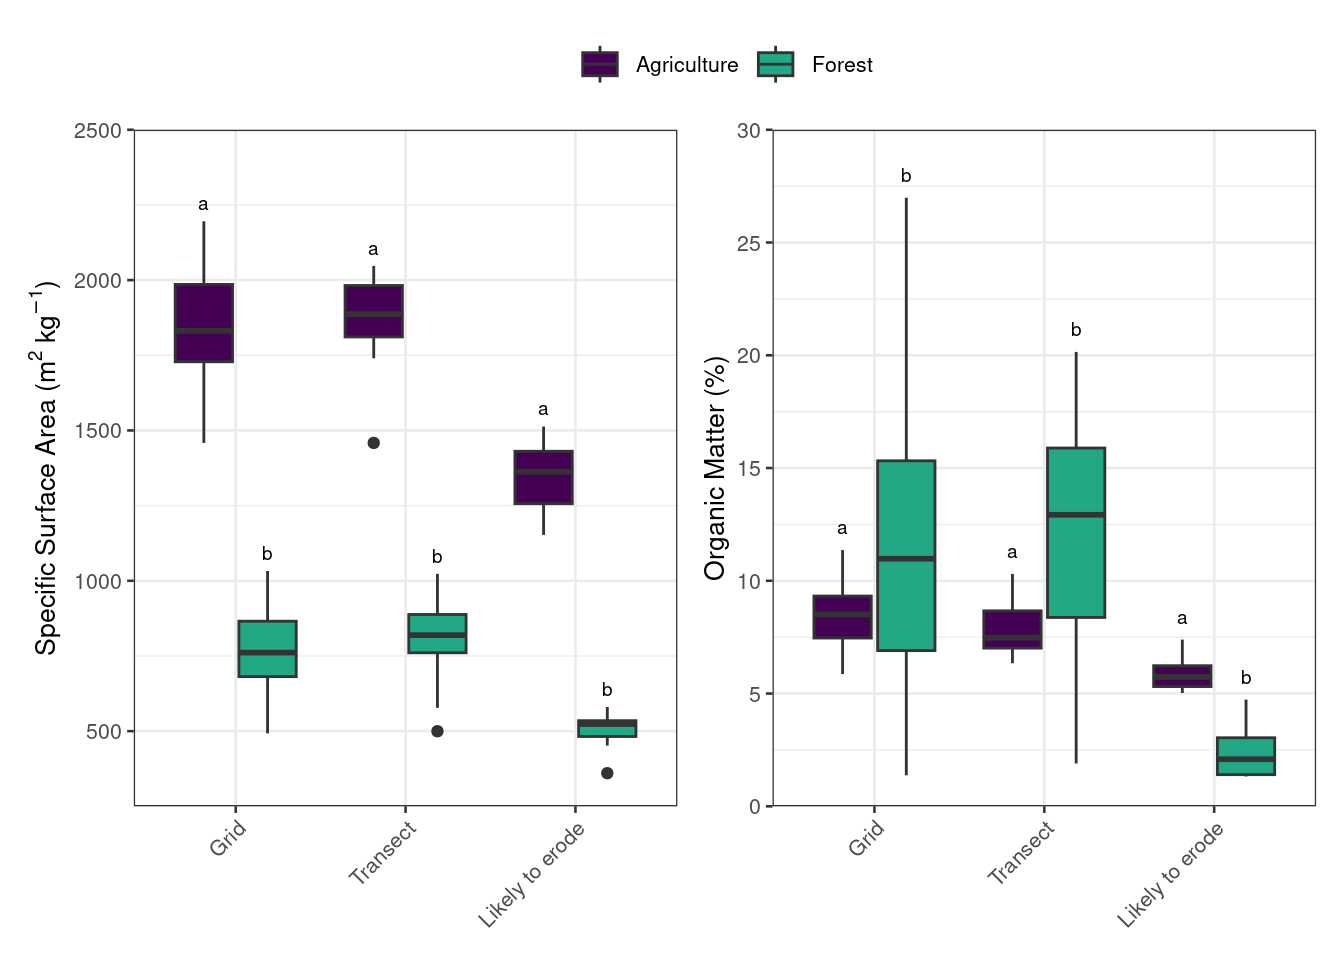
\includegraphics{index_files/figure-latex/notebooks-PSA_OM-fig-ssasom-plot-output-2.png}

}

\caption{\label{fig-ssasom-plot}Specific surface area and soil organic
matter for the agricultural and forested sites as determined by the
three sampling designs.}

\end{figure}%

\textsubscript{Source:
\href{https://alex-koiter.github.io/sampling-design-manuscript/notebooks/PSA_OM-preview.html\#cell-fig-ssasom-plot}{Plotting
SSA and SOM}}

In comparing the sampling designs on characterizing colour properties at
the two sites six (\emph{X, Y, Z, L, G, B}) and three (\emph{x, u*, a*})
colour coefficients showed no significant differences between the
sampling designs for the agricultural and forested sites, respectively
(Figure~\ref{fig-dunns-test}). The post-hoc test showed that there were
no significant differences between the grid and transect sampling
designs at both sites for all colour fingerprints
(Figure~\ref{fig-dunns-test}). There were also no difference between the
likely to erode and transect sampling designs for the colour properties
\emph{R} and \emph{h*} (Figure~\ref{fig-dunns-test}).

At both sites no significant differences (p \textgreater{} 0.05) were
found between the different sampling designs for five geochemical
elements (Ce, Co, La, Mn, Te, Y) and an additional ten (Ba, Bi, Ca, Cs,
Hg, K, Pb, Rb, Se, Sr) and eight (Fe, Hf, Li, Mn, Ni, Sb, Sc, Tl)
geochemical elements for the agricultural and forested sites,
respectively (Figure~\ref{fig-dunns-test}). For the forest site the
post-hoc test showed that there were no significant differences between
the grid and transect sampling designs for all geochemical fingerprints.
In contrast, there were significant difference between the other two
comparisons with the exceptions of In and Zr
(Figure~\ref{fig-dunns-test}). Similarly, within the agricultural sites
there are 18 geochemical fingerprints not show no significant
differences between the grid and transect sampling designs, nine between
transect and likely to erode, and four between the grid and likely to
erode (Figure~\ref{fig-dunns-test}).

\begin{figure}[H]

\centering{

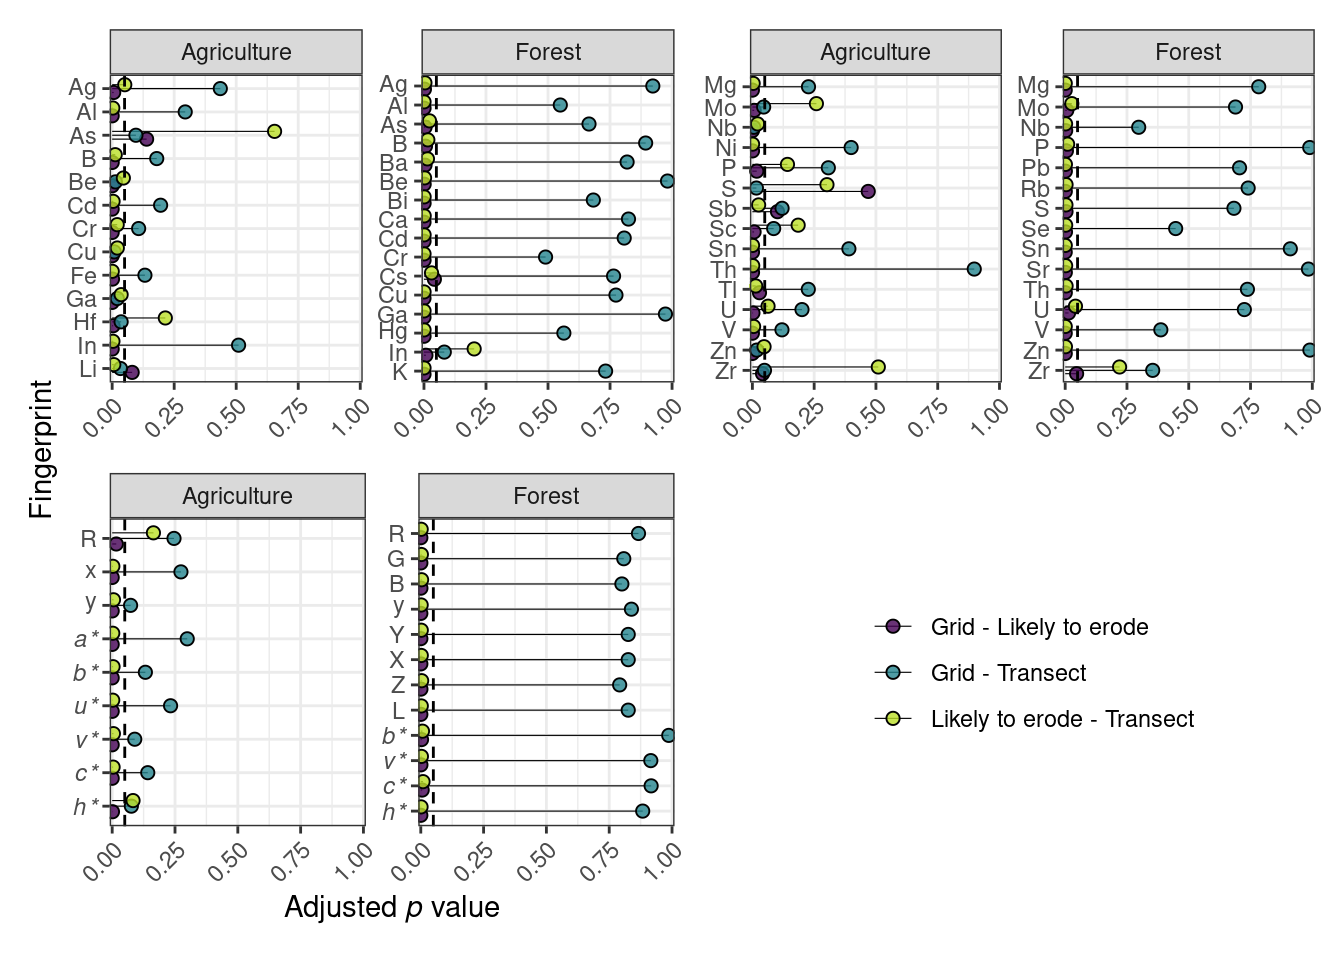
\includegraphics{index_files/figure-latex/notebooks-kruskal-fig-dunns-test-output-1.png}

}

\caption{\label{fig-dunns-test}Results for the pair-wise Dunn's post-hoc
test to determine differences in fingerprint properties between the
three sampling designs for each site. Dashed line represents an α value
of 0.05. Fingerprints that showed no significant differences (p value
\textgreater{} 0.05) following the Kruskal Wallis test are not
included.}

\end{figure}%

\textsubscript{Source:
\href{https://alex-koiter.github.io/sampling-design-manuscript/notebooks/kruskal-preview.html\#cell-fig-dunns-test}{Testing
for differences between sites using three different sampling}}

In assessing the correlation between colour and SSA there were clear
differences between sites and sampling design
(\quartosuppplotref{suppplot-supfig1} and
\quartosupptabref{supptab-corr-summary}). Within the likely to erode
design the correlation was found to be significant for 12 out of the 15
colour coefficients only when the data was combined across both sites.
For the agricultural site only the grid design detected significant
correlations. Interestingly, the direction and magnitude of the
correlations depended on the sampling design used and/or if the data was
grouped by site or combined. For example, u* demonstrates a much higher
degree of correlation when the data is pooled across the two sites as
compared to assessing each site independently. Overall, the colour
properties showed a higher number of significant correlations with SOM
as compared to SSA regardless of sampling design or how the data was
grouped (\quartosuppplotref{suppplot-supfig2} and
\quartosupptabref{supptab-corr-summary}). Similar to the correlations
with SSA, the number of significant correlations with SOM within the
likely to erode design was greatest when the data was combined. The
magnitude and direction of the correlations between colour properties
and SOM is also variable across sampling designs and the grouping of the
data. For example, the colour coefficient x demonstrates no significant
correlations when each site is considered independently but the combined
data demonstrates a positive but weak correlation (r\textsuperscript{2}
\textless{} 0.4) for the grid and transect designs and a stronger and
negative correlation (r\textsuperscript{2} = -0.75) for the likely to
erode design.

Similar to the relation between colour and SSA, there were differences
between sites and sampling designs in assessing the influence of grain
size on the concentration of geochemical elements
(\quartosuppplotref{suppplot-supfig3} and
\quartosupptabref{supptab-corr-summary}). Using the likely to erode
sampling design there were few significant correlations when
investigated independently for the agricultural and forested sites
independently; however, pooling the data across both sites increase the
number of observed significant correlations. The direction of the
correlation between concentration and SSA was mostly positive when the
data was combined but more variable when each site was assessed
independently. The correlation between geochemical concentration and SOM
shares some similarities as compared to the correlation with SSA
(\quartosuppplotref{suppplot-supfig4} and
\quartosupptabref{supptab-corr-summary}). However, one observed
difference is that when the data is pooled across the sites the likely
to erode sampling design typically had a positive correlation between
SOM and concentration, whereas the other two sampling designs were
typically negatively correlated.

The correlations (i.e., slope) between fingerprints and SSA and SOM also
varies widely between fingerprint, site, and sampling designs used to
characterize the soil properties (Figure~\ref{fig-colour-corr} and
Figure~\ref{fig-geochem-corr}). For example, the relation between the
concentration of Al and SSA demonstrates a good example where combining
data from both sites may be preferable to an assessment on each site
independently. In contrast, the Tl data suggests that a that site/land
use specific assessment may be more appropriate
(Figure~\ref{fig-geochem-corr}). However, a complete assessment of the
role of particle size and organic matter on the fingerprinting method
requires information on downstream sediment as well.

\begin{figure}[H]

\centering{

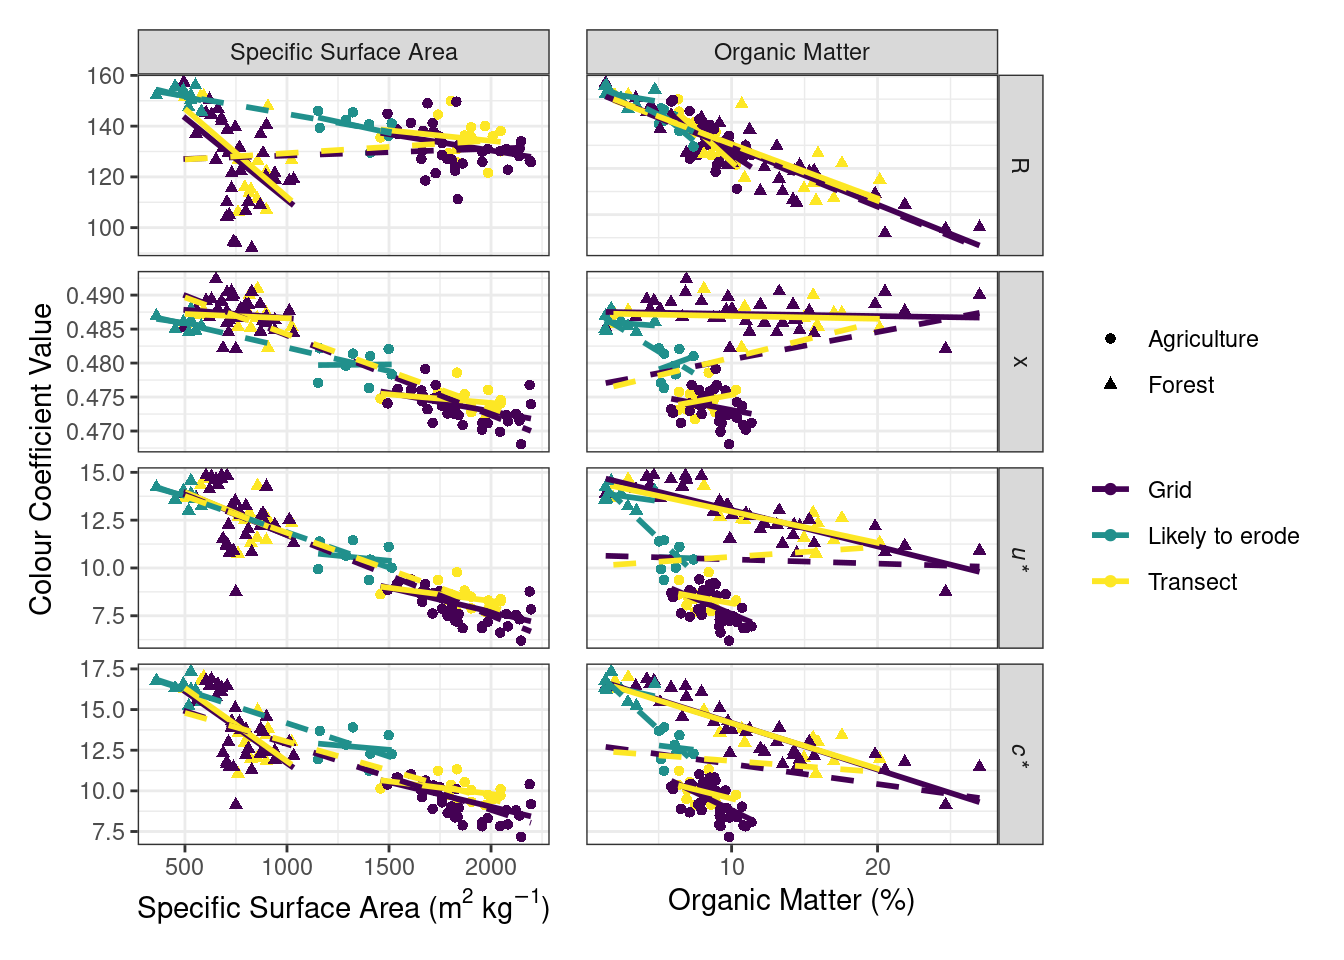
\includegraphics{index_files/figure-latex/notebooks-correlation-fig-colour-corr-output-2.png}

}

\caption{\label{fig-colour-corr}Exploring the relation between select
colour coefficients and specific surface area and soil organic matter
content. Solid lines indicate linear relation for each site and sampling
design independently and dashed lines indicate linear relation for each
sampling design with data combined across both sites.}

\end{figure}%

\textsubscript{Source:
\href{https://alex-koiter.github.io/sampling-design-manuscript/notebooks/correlation-preview.html\#cell-fig-colour-corr}{Correlations
between soil colour and geochemical properties and SSA}}

\begin{figure}[H]

\centering{

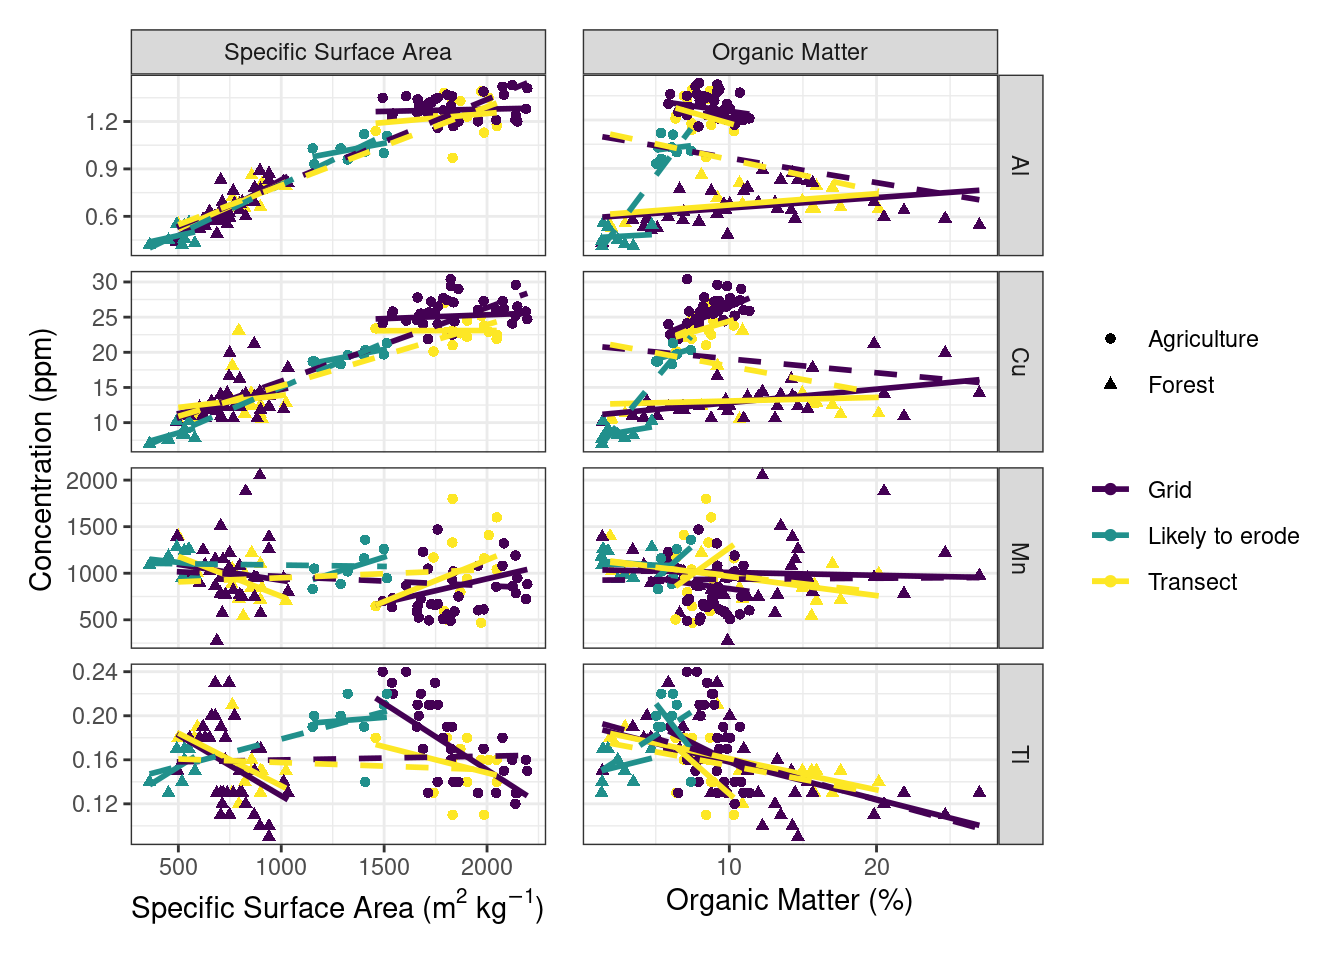
\includegraphics{index_files/figure-latex/notebooks-correlation-fig-geochem-corr-output-2.png}

}

\caption{\label{fig-geochem-corr}Exploring the relation between select
geochemical concentrations and specific surface area and soil organic
matter content. Solid lines indicate linear relation for each site and
sampling design independently and dashed lines indicate linear relation
for each sampling design with data combined across both sites.}

\end{figure}%

\textsubscript{Source:
\href{https://alex-koiter.github.io/sampling-design-manuscript/notebooks/correlation-preview.html\#cell-fig-geochem-corr}{Correlations
between soil colour and geochemical properties and SSA}}

\subsection{Source discrimination and
apportionment}\label{source-discrimination-and-apportionment}

A total of 58, 50, and 12 fingerprint properties passed the range test
for the grid, transect, and likely to erode designs, respectively
(Table~\ref{tbl-range}). For all the colour fingerprints at least one of
the virtual mixtures fell outside of the IQR for the likely to erode
sources resulting in their elimination from further analysis. The Mann
Whitney U-test (p-value \textless{} 0.01) further reduced the number of
fingerprints for the grid and transect to 49 and 33, respectively and
number remained the same for the likely to erode sampling design
(tbl-MW). The stepwise DFA further reduced the number of fingerprints to
16, three, and three grid, transect, and likely to erode designs,
respectively (Table~\ref{tbl-DFA}). Of note is that the geochemical
concentrations of Li and Fe as well as the colour coefficient \emph{a*}
which were selected as the first, second, or third variables in the DFA
in two of the three sampling designs. The fingerprints selected for all
three sampling designs classified 100\% of the source samples correctly
(Table~\ref{tbl-DFA}). Using the design specific mixtures a greater
number of fingerprints passed the range and Mann Whitney U test;
however, the same fingerprints were ultimately selected for all three
designs by the DFA with 100\% classification
(\quartosupptabref{supptab-range-test}, \quartosupptabref{supptab-KW-test},
\quartosupptabref{supptab-DFA}).

\begin{longtable}[]{@{}
  >{\raggedright\arraybackslash}p{(\columnwidth - 2\tabcolsep) * \real{0.3472}}
  >{\raggedright\arraybackslash}p{(\columnwidth - 2\tabcolsep) * \real{0.6528}}@{}}
\caption{Fingerprint properties that passed the range test for
conservative behavior for each sampling
approach.}\label{tbl-range}\tabularnewline
\toprule\noalign{}
\begin{minipage}[b]{\linewidth}\raggedright
Sampling design
\end{minipage} & \begin{minipage}[b]{\linewidth}\raggedright
Fingerprinting properties
\end{minipage} \\
\midrule\noalign{}
\endfirsthead
\toprule\noalign{}
\begin{minipage}[b]{\linewidth}\raggedright
Sampling design
\end{minipage} & \begin{minipage}[b]{\linewidth}\raggedright
Fingerprinting properties
\end{minipage} \\
\midrule\noalign{}
\endhead
\bottomrule\noalign{}
\endlastfoot
Grid & Ag Al As Ba Be Bi Ca Ca Cd Ce Co Cr Cu Fe Ga Hf Hg In K K La Li
Mg Mn Nb Ni P Pb Rb S Sb Sb Sc Se Sn Sr Th Tl U V Y Zn Zr R G B \emph{x*
y* Y X Z L a* b* u* v* c* h*} \\
Transect & Ag Al As Ba Be Ca Cd Ce Co Cr Cs Fe Ga Hg In La Mg Mn Mo Ni P
Pb Rb S Sb Sc Se Sn Sr Te Th Tl U V Y Zn R G B \emph{x* y* Y X Z L a* b*
u* v* c* h*} \\
Likely to erode & Ba Bi Co Cs Li Mo Pb S Sn Tl U Zr \\
\end{longtable}

\begin{longtable}[]{@{}
  >{\raggedright\arraybackslash}p{(\columnwidth - 2\tabcolsep) * \real{0.3472}}
  >{\raggedright\arraybackslash}p{(\columnwidth - 2\tabcolsep) * \real{0.6528}}@{}}
\caption{Fingerprint properties that passed the Mann Whitney test for
each sampling approach..}\label{tbl-MW}\tabularnewline
\toprule\noalign{}
\begin{minipage}[b]{\linewidth}\raggedright
Sampling design
\end{minipage} & \begin{minipage}[b]{\linewidth}\raggedright
Fingerprinting properties
\end{minipage} \\
\midrule\noalign{}
\endfirsthead
\toprule\noalign{}
\begin{minipage}[b]{\linewidth}\raggedright
Sampling design
\end{minipage} & \begin{minipage}[b]{\linewidth}\raggedright
Fingerprinting properties
\end{minipage} \\
\midrule\noalign{}
\endhead
\bottomrule\noalign{}
\endlastfoot
Grid & Ag Al As Be Bi Ca Cd Ce Co Cr Cs Cu Fe Ga Hf Hg In K La Li Mg Nb
Ni Rb S Sb Sc Se Sn Sr Te Th U V Y Zr \emph{B G x Y X Z L a* b* u* v* c*
h*} \\
Transect & Ag Al As Be Ca Cd Ce Co Cr Cs Fe Ga In La Ni S Sb Sc Se Sn Sr
Te U V Y \emph{B} \emph{x Z a* b* u* c* h*} \\
Likely to erode & Ba Bi Co Cs Li Mo Pb Sn Tl U \\
\end{longtable}

\begin{table}

\caption{\label{tbl-DFA}Results of the stepwise DFA for each sampling
approach including the percent of samples correctly classified for each
site.}

\begin{minipage}{\linewidth}

\subcaption{\label{tbl-first}Grid sampling design}

\centering{

\begin{tabular}{llll}
\toprule
Composite fingerprint & Wilks' lambda & Agriculture & Forest\\
\midrule
Li & 0.062 & 100 & 100\\
Li + a* & 0.044 & 100 & 100\\
Li + a* + Fe & 0.028 & 100 & 100\\
Li + a* + Fe + Co & 0.023 & 100 & 100\\
Li + a* + Fe + Co + Hg & 0.022 & 100 & 100\\
Li + a* + Fe + Co + Hg + x & 0.019 & 100 & 100\\
Li + a* + Fe + Co + Hg + x + Cs & 0.018 & 100 & 100\\
Li + a* + Fe + Co + Hg + x + Cs + La & 0.015 & 100 & 100\\
Li + a* + Fe + Co + Hg + x + Cs + La + Ni & 0.013 & 100 & 100\\
Li + a* + Fe + Co + Hg + x + Cs + La + Ni +Nb & 0.013 & 100 & 100\\
Li + a* + Fe + Co + Hg + x + Cs + La + Ni + Nb +
h* & 0.012 & 100 & 100\\
Li + a* + Fe + Co + Hg + x + Cs + La + Ni + Nb + h* +
b* & 0.011 & 100 & 100\\
Li + a* + Fe + Co + Hg + x + Cs + La + Ni + Nb + h* + b* +
Rb & 0.011 & 100 & 100\\
Li + a* + Fe + Co + Hg + x + Cs + La + Ni + Nb + h* + b* + Rb +
Ca & 0.010 & 100 & 100\\
Li + a* + Fe + Co + Hg + x + Cs + La + Ni + Nb + h* + b* + Rb + Ca +
Sr & 0.009 & 100 & 100\\
Li + a* + Fe + Co + Hg + x + Cs + La + Ni + Nb + h* + b* + Rb + Ca + Sr
+ c* & 0.009 & 100 & 100\\
\bottomrule
\end{tabular}

}

\end{minipage}%
\newline
\begin{minipage}{\linewidth}

\subcaption{\label{tbl-second}Transect sampling design}

\centering{

\begin{tabular}{llll}
\toprule
Composite fingerprint & Wilks' lambda & Agriculture & Forest\\
\midrule
Fe & 0.052 & 100 & 100\\
Fe + a* & 0.025 & 100 & 100\\
Fe + a* + Co & 0.009 & 100 & 100\\
\bottomrule
\end{tabular}

}

\end{minipage}%
\newline
\begin{minipage}{\linewidth}

\subcaption{\label{tbl-third}Likely to erode sampling design}

\centering{

\begin{tabular}{llll}
\toprule
Composite fingerprint & Wilks' lambda & Agriculture & Forest\\
\midrule
Li & 0.024 & 100 & 100\\
Li + U & 0.011 & 100 & 100\\
Li + U + Bi & 0.008 & 100 & 100\\
\bottomrule
\end{tabular}

}

\end{minipage}%

\end{table}%

The subsequent principal component analysis (PCA) illustrated that the
geochemical and colour composition in the agricultural field,
considering the three sampling approaches, was different than the
forested site (Figure~\ref{fig-pcaplot} and
\quartosuppplotref{suppplot-supfig5}). The first principal component for
the grid sampling demonstrate a similar magnitude in loadings where
\emph{a*}, \emph{b*}, \emph{c*}, and \emph{x*} are negative and Co, Fe,
La, Li, Nb, Ni, Sr, and \emph{h*} are positive. The second principal
component the sites are differentiated mostly by \emph{b*}, \emph{c*},
and Hg. For the transect sampling, first principal component
demonstrated a similar magnitude in loadings for all three fingerprints
(\emph{a*}, Co, and Fe) while the second principal component are
differentiated by \emph{a*} and Co.~Similarly, the first principal
component for the likely to erode design demonstrated a similar
magnitude in loadings for all three fingerprints (Bi, Li, and U) while
the second principal component are primarily differentiated by U.

\begin{figure}[H]

\centering{

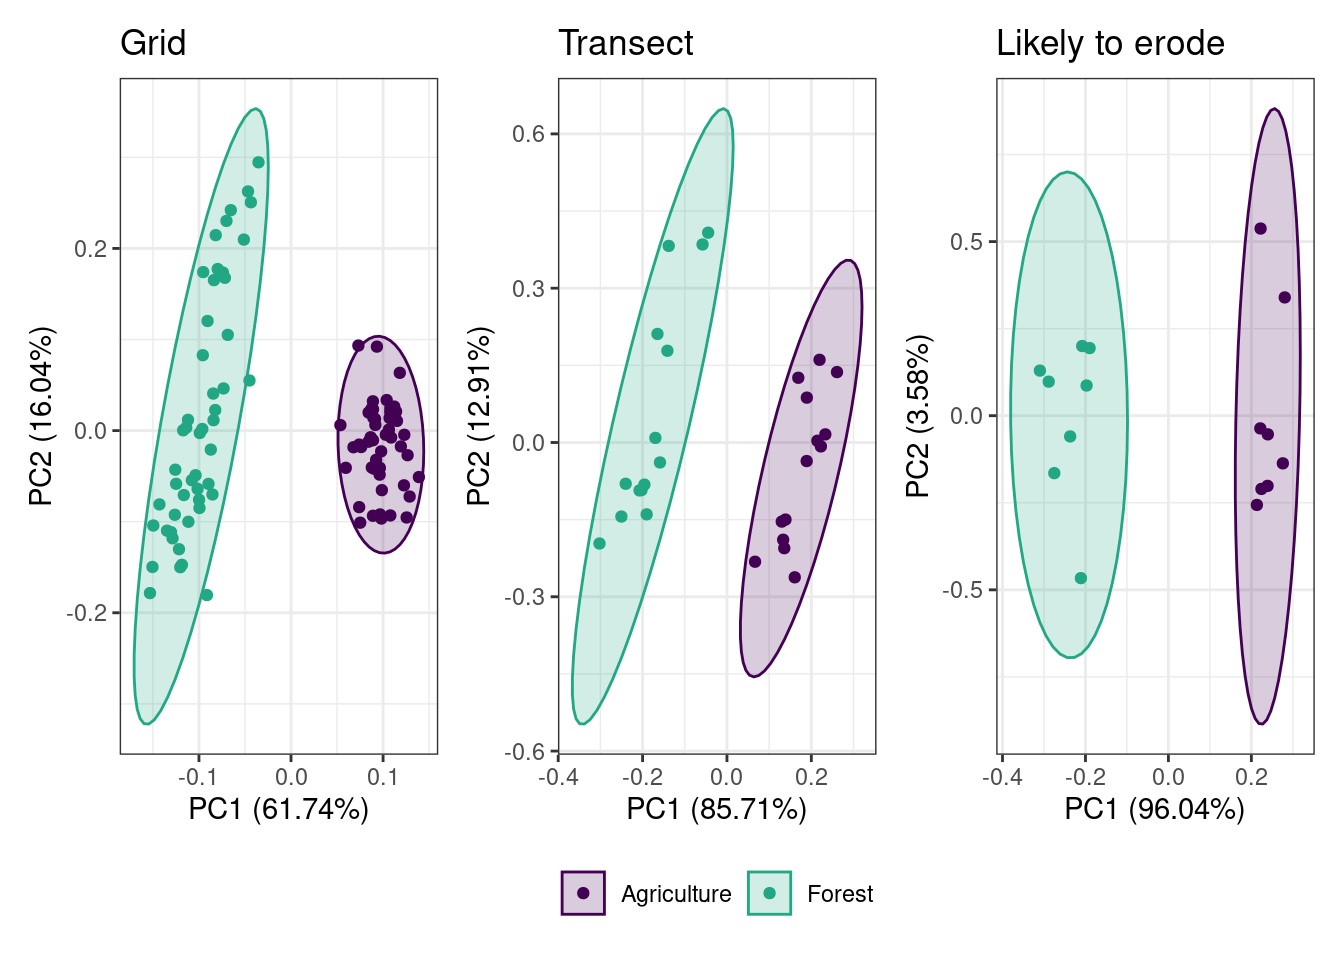
\includegraphics{index_files/figure-latex/notebooks-Tracer_selection-fig-pcaplot-output-1.png}

}

\caption{\label{fig-pcaplot}Principle component analysis demonstrating
the discriminatory ability for the selected fingerprints for the three
sampling designs.}

\end{figure}%

\textsubscript{Source:
\href{https://alex-koiter.github.io/sampling-design-manuscript/notebooks/Tracer_selection-preview.html\#cell-fig-pcaplot}{Tracer
selection using composite mixtures}}

Results of means and standard deviations of all the fingerprints that
were included in the MixSIAR runs are illustrated in
Figure~\ref{fig-sdplot-test}. The relative contributions of potential
sources to the virtual mixtures for each sampling design are shown in
Figure~\ref{fig-unmixing-plot}. For all three sampling designs the
difference between the virtual mixture and the modeled proportions were
larger towards when the differences between the contributions was large
(e.g., 0\% forest, 100\% agriculture)
(Figure~\ref{fig-unmixing-diff-plot}). The maximum median absolute
difference between the virtual mixtures and the modeled proportions was
7.7, 7.8, and 8.9\% for the grid, transect, and likely to erode sampling
design respectively. The mixing model results for the design specific
mixtures simulation were similar (Figs.
\quartosuppplotref{suppplot-supfig6} and
\quartosuppplotref{suppplot-supfig7}). The uncertainty metrics were
generally similar among the three sampling designs, with the exception
of the W95 (0.025-0.975 quantile width) for the grid was smaller than
the other designs (Table~\ref{tbl-model-performance}). In terms of the
uncertainty and performance metrics the grid was marginally better.
Lastly, the contingency metrics were generally similar among the three
sampling designs, with the exception of the CSI95 (Critical success
index) for the grid sampling where the hit rate for the 95\% interval
was higher (\textasciitilde10 to 2\%). The CRPS showed a U-shaped
response with higher values at the 0 and 100\% contributions
(\quartosuppplotref{suppplot-supfig8}) Overall there was a high degree
of similarity in model evaluation metrics. Using the design specific
mixtures the modeled apportionment and model performance metrics are
similar to the combined mixtures
(\quartosupptabref{supptab-model-performance} and
\quartosuppplotref{suppplot-supfig9}).

\begin{figure}[H]

\centering{

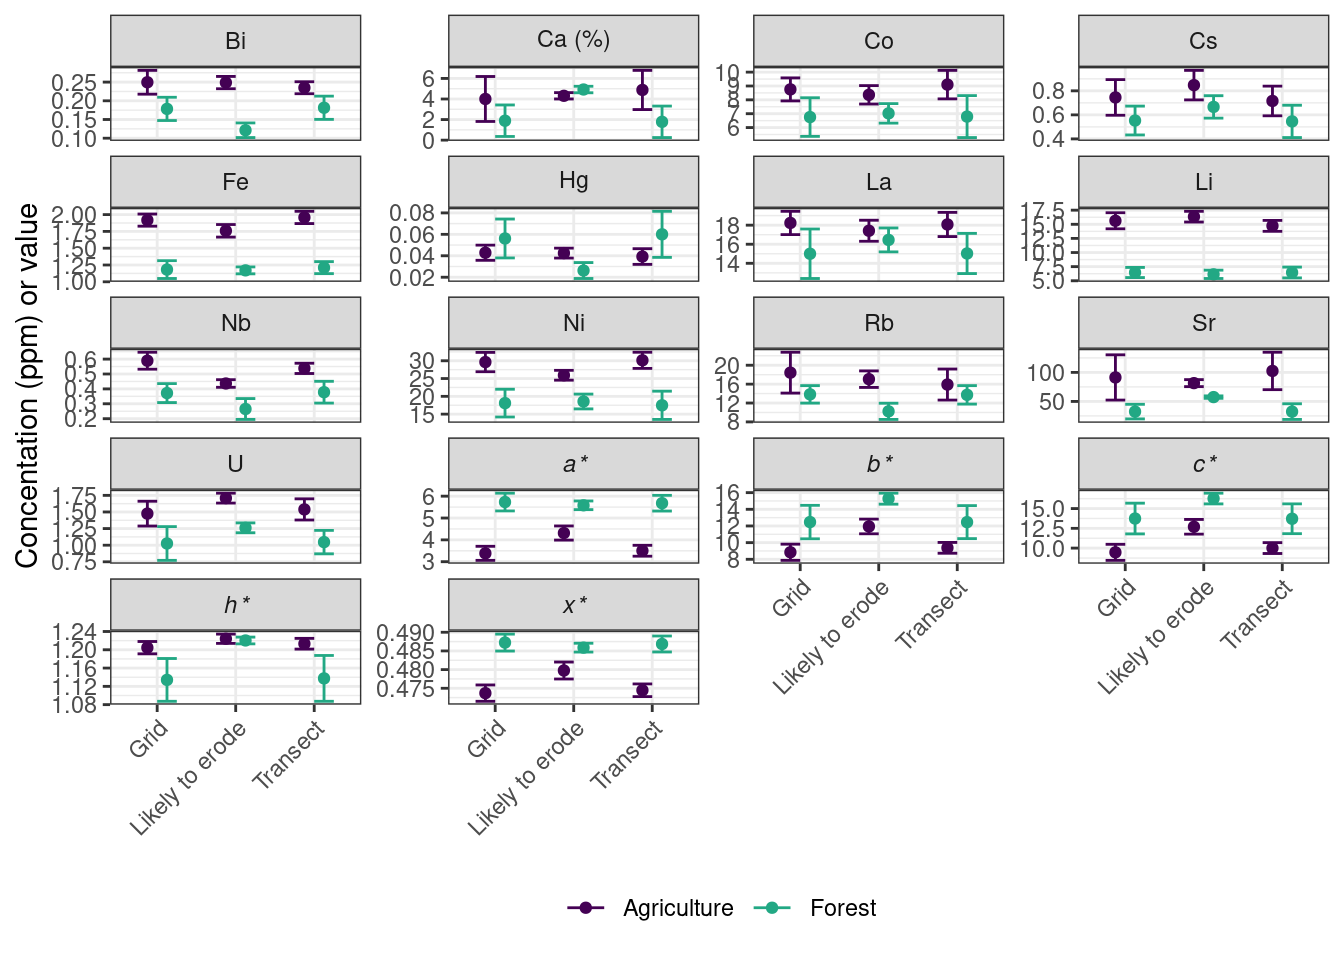
\includegraphics{index_files/figure-latex/notebooks-Tracer_selection-fig-sdplot-test-output-1.png}

}

\caption{\label{fig-sdplot-test}Means and standard deviations of the
fingerprints used in the mixing model.}

\end{figure}%

\textsubscript{Source:
\href{https://alex-koiter.github.io/sampling-design-manuscript/notebooks/Tracer_selection-preview.html\#cell-fig-sdplot-test}{Tracer
selection using composite mixtures}}

\begin{figure}[H]

\centering{

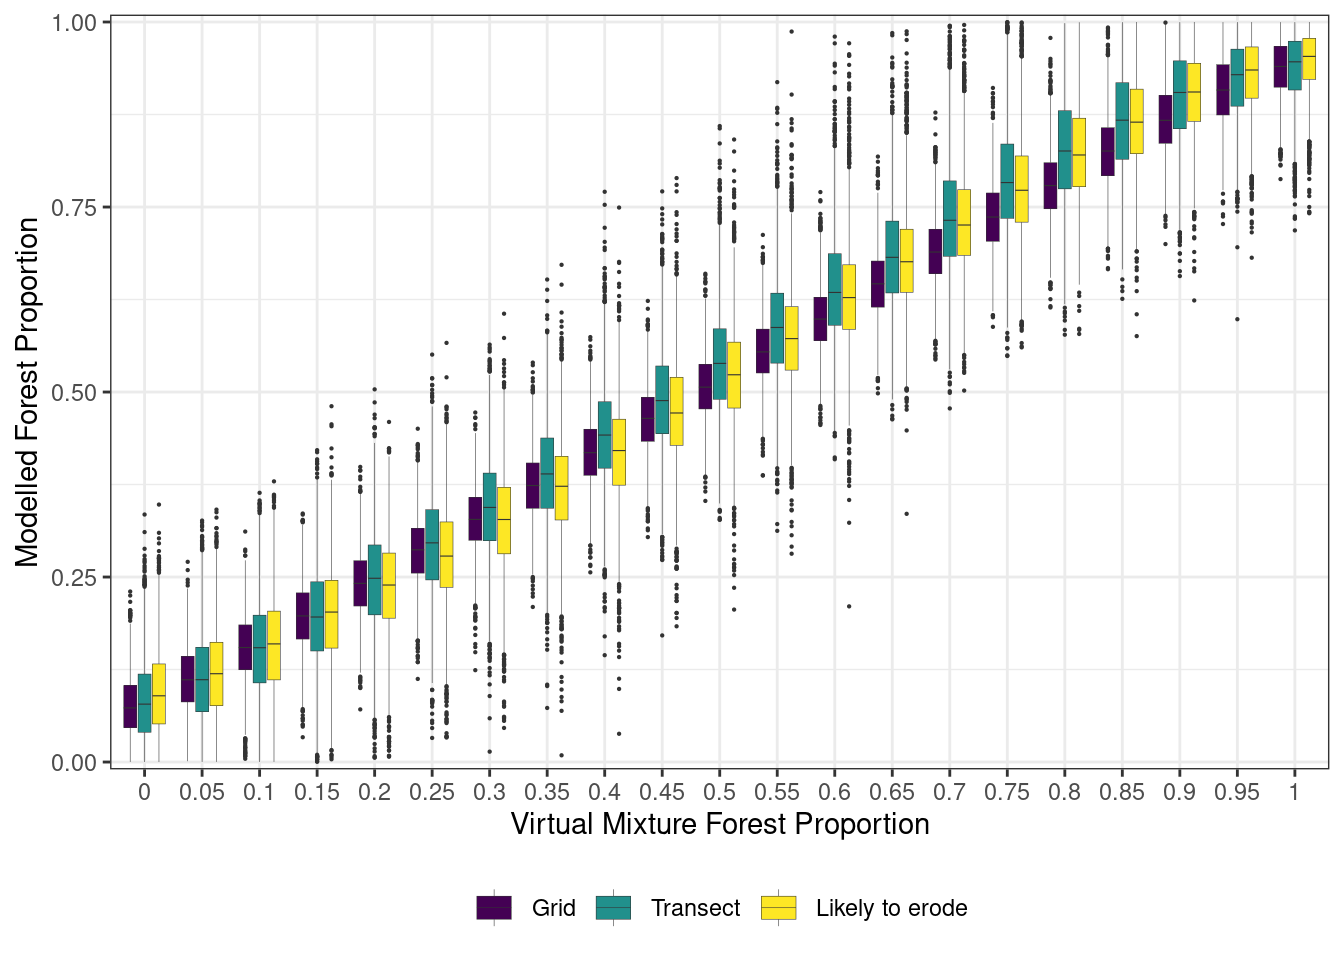
\includegraphics{index_files/figure-latex/notebooks-Mixture_plots_all-fig-unmixing-plot-output-1.png}

}

\caption{\label{fig-unmixing-plot}Comparison of the posterior
distribution of the modeled proportion of forest source to the
proportion of forest source in the virtual mixtures for each of the
three sampling designs.}

\end{figure}%

\textsubscript{Source:
\href{https://alex-koiter.github.io/sampling-design-manuscript/notebooks/Mixture_plots_all-preview.html\#cell-fig-unmixing-plot}{MixSIAR
results plotting and model performance - composite mixtures}}

\begin{figure}[H]

\centering{

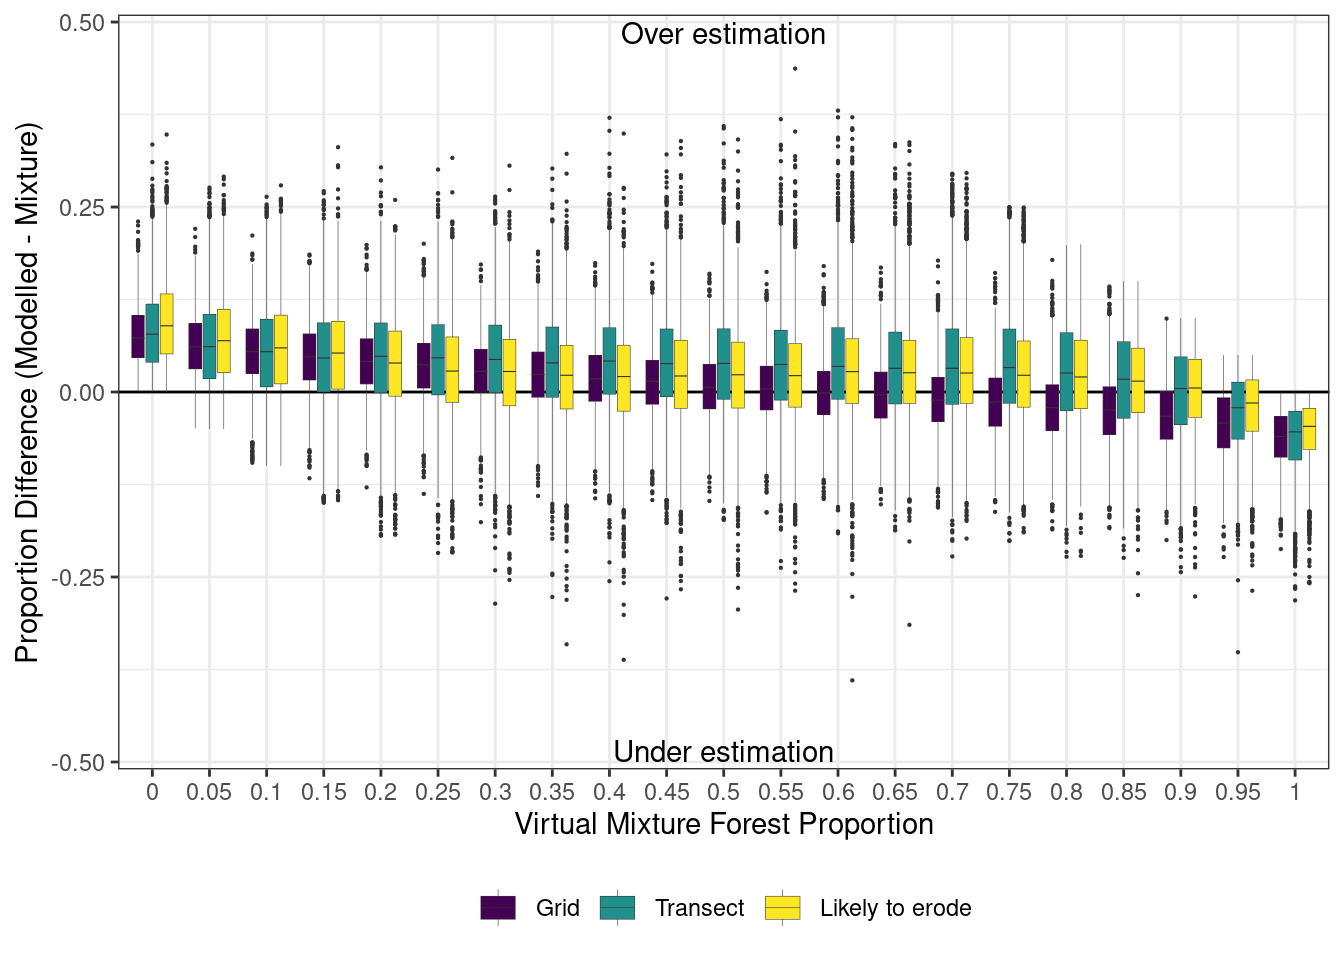
\includegraphics{index_files/figure-latex/notebooks-Mixture_plots_all-fig-unmixing-diff-plot-output-1.png}

}

\caption{\label{fig-unmixing-diff-plot}Differences in the proportions
between modeled and virtual mixtures.}

\end{figure}%

\textsubscript{Source:
\href{https://alex-koiter.github.io/sampling-design-manuscript/notebooks/Mixture_plots_all-preview.html\#cell-fig-unmixing-diff-plot}{MixSIAR
results plotting and model performance - composite mixtures}}

\begin{longtable}[]{@{}ccccccc@{}}

\caption{\label{tbl-model-performance}Model evaluation metrics grouped
by sampling design and source.}

\tabularnewline

\toprule\noalign{}
Parameter & Grid Agriculture & Grid Forest & Transect Agriculture &
Transect Forest & Likely to erode Agriculture & Likely to erode
Forest \\
\midrule\noalign{}
\endhead
\bottomrule\noalign{}
\endlastfoot
\multicolumn{7}{@{}c@{}}{%
Residuals} \\
MAE50 & 0.01 & 0.01 & 0.02 & 0.02 & 0.02 & 0.02 \\
MAE95 & 0.00 & 0.00 & 0.00 & 0.00 & 0.00 & 0.00 \\
ME50 & 0.00 & 0.00 & 0.00 & 0.00 & 0.00 & 0.00 \\
ME95 & 0.00 & 0.00 & 0.00 & 0.00 & 0.00 & 0.00 \\
\multicolumn{7}{@{}c@{}}{%
Performance} \\
NSE50 & 0.99 & 0.99 & 0.98 & 0.98 & 0.98 & 0.98 \\
NSE95 & 1.00 & 1.00 & 1.00 & 1.00 & 1.00 & 1.00 \\
CRPS & 0.02 & 0.02 & 0.03 & 0.03 & 0.02 & 0.02 \\
\multicolumn{7}{@{}c@{}}{%
Contingency} \\
CSI50 & 0.92 & 0.93 & 0.86 & 0.90 & 0.88 & 0.89 \\
CSI95 & 0.86 & 0.82 & 0.75 & 0.80 & 0.77 & 0.78 \\
HR50 & 0.99 & 0.98 & 0.99 & 0.98 & 0.98 & 0.99 \\
HR95 & 1.00 & 1.00 & 1.00 & 1.00 & 1.00 & 1.00 \\
\multicolumn{7}{@{}c@{}}{%
Uncertainty} \\
W50 & 0.06 & 0.06 & 0.09 & 0.09 & 0.09 & 0.09 \\
W95 & 0.18 & 0.18 & 0.27 & 0.27 & 0.26 & 0.26 \\
P50 & 0.25 & 0.25 & 0.23 & 0.27 & 0.24 & 0.26 \\
P95 & 0.47 & 0.48 & 0.44 & 0.51 & 0.45 & 0.50 \\

\end{longtable}

\textsubscript{Source:
\href{https://alex-koiter.github.io/sampling-design-manuscript/notebooks/Mixture_plots_all-preview.html\#cell-tbl-model-performance}{MixSIAR
results plotting and model performance - composite mixtures}}

\section{Discussion}\label{discussion}

\subsection{Characterization of soil
properties}\label{characterization-of-soil-properties-1}

SOM can exert a strong control on the concentration and values for
geochemical- and colour-based fingerprints; and therefore, an important
factor to consider when evaluating the results from sediment source
fingerprinting studies \citep{horowitz1991, viscarrarossel2009}. Results
from this study indicate that there are differences in means for SOM
content, and the amount of variation is different among the three
sampling approaches and land uses (Figure~\ref{fig-ssasom-plot}).
Results from the grid and transect sampling approaches illustrate that
the amount of SOM in surface soil was lower at the agricultural site
compared to the forested site. The lower SOM content at the agricultural
site is likely due to the regular harvesting of biomass and mixing of
soil due to tillage. The conversion of native ecosystems to agricultural
land uses generally results in a net loss of SOM as tillage increases
the contact between soil and biomass and improves soil aeration
resulting in higher rates of decomposition \citep{brady2001}. However,
results from the likely to erode sampling approach indicated that the
SOM was higher at the agricultural site compared to the forested site.
This difference may be due to soil forming factors, including hydrology
(i.e., lower slope positions) and the accumulation of organic-rich
particles due to erosion. Similarly, natural factors may also reduce the
accumulation or dilute the SOM in the forested site as the location of
the likely to erode is situated within a floodplain, and the deposition
of coarse-grained and organic-poor sediment (i.e., shale from the
Manitoba Escarpment) have been observed following flooding.

The grid, transect, and likely to erode sampling designs all showed
differences in grain size (i.e., SSA) in the surface soil between the
forested and agriculture sites. There is little evidence that land use
practices have a direct impact on the grain size (i.e., rate of clay
formation); however, geomorphic processes both local and regional may
impact the grain size. Regionally, the forested site is closer to the
base of the escarpment and coarser-grained material eroded within the
escarpment (i.e., deeply incised stream) is likely being deposited near
at the apex of the alluvial fan, which lies in the lacustrine deposits
of glacial Lake Agassiz \citep{mcginn1979}. Locally, wind, water, and
tillage erosion, and localized flooding, may exert a strong influence on
the spatial pattern and range in grain size. For example, the likely to
erode material sampled at both sites function as an intermediate
storage, a sink of sediment derived from upslope and a source of
sediment to the adjacent channel or surface drain and may explain the
observed coarse grained material near the channel environment. This
study highlights the importance the sampling strategy can have on
characterizing both grain size and SOM properties.

In characterizing the geochemical concentration and colour properties of
the two sites, this study demonstrated the sampling design used had an
impact. Fingerprint properties that exhibit strong spatial patterns due
to environmental gradients (e.g., soil moisture) and geomorphic
processes (e.g., erosional and depositional areas)
\citep{hoffmann2009, borch2010} are more likely more sensitive to the
sampling design (i.e., significant differences between sampling designs)
while fingerprints that exhibit no spatial patterns are likely to be
less sensitive. The comparison between the grid and transect sampling
designs resulted in the fewest differences in fingerprinting properties
(Figure~\ref{fig-dunns-test}). This is likely due to the fact that the
transect is a subset of the larger grid. The samples collected from the
likely to erode had a unique fingerprinting properties as compared to
the other two sampling designs (Figure~\ref{fig-dunns-test} and
Figure~\ref{fig-sdplot-test}). The material from likely to erode
sampling is normally collected at the edge of the field or close to the
stream where the hydrologic regime is different than up-slope positions
and is typically characterized by an overall higher moisture status and
a fluctuating water table.

The redox conditions often found in these areas can facilitate the
precipitation of some minerals (e.g., Zinc Sulphide), increase the
solubility and mobility of certain elements (e.g., As, Fe and Mn)
\citep{dulaing2010, rinklebe2016}. For example, at the agricultural site
the concentration of Fe was significantly lower for the likely erode
samples compared to the other two designs (Figure~\ref{fig-dunns-test}
and Figure~\ref{fig-sdplot-test}) and may be related to the hydrology of
the lower slope position. However, grain size and SOM is often
correlated to geochemical concentrations due to their high SSA and
reactivity, and the lower Fe concentration observed may be related to
the coarser grain size and lower SOM observed
(Figure~\ref{fig-ssasom-plot}). In contrast, Mn should follow a similar
pattern but there was no difference in Mn concentration detected between
the three sampling designs. Differentiating between the role of
pedogenic and grain size of the concentration of Fe, Mn or other
geochemical properties across the landscape is difficult and requires
additional study that is typically outside the scope of most
fingerprinting studies. Similarly, the observed differences in both SSA
and SOM (Figure~\ref{fig-ssasom-plot}) are likely driving the observed
difference in colour properties between sites (Table~\ref{tbl-MW}) and
between the likely to erode and the other two designs
(Figure~\ref{fig-dunns-test}) as the higher SOM and SSA typically result
in darker brown/black colours \citep{viscarrarossel2006}. Spatial
interpolation the fingerprint data combined with landscape attributes
derived from topographic information would identify whether spatial
patterns exist and if they relate to landforms. This will help identify
the underlying processes that create the observed patterns and further
inform sampling design and fingerprint selection.

Accurate characterization of sediment sources is a key component
underlying the sediment source fingerprinting approach. Key to achieving
this is using an appropriate sampling approach as to not introduce
sampling bias and provide an accurate estimation of the mean and
variance for each source. Sampling designs are sensitive to fingerprint
variance and heterogeneity. Identifying fingerprints that are more
homogeneous within a given source would be beneficial as there is less
potential for an observed difference (or no difference) between sources
to be an artifact of sampling design and not underlying geology/land
use. From a practical perspective, there is often little information on
the variance and heterogeneity of fingerprints both within and between
sources prior to sampling. However, this study investigated a single
location for each potential source of sediment and the variability of
these fingerprints between different locations across the watershed
remains unquantified and a research priority. Due to time and cost
constraints, there is often a trade-off between the number of samples at
a given location and the number of locations throughout the watershed.
Observations at both scales would provide insight into the distribution
of fingerprint properties. The impact of different sampling designs at
the larger watershed is also an important research question that should
be addressed in future studies.

Information on grain size and organic matter content is needed for
watershed and environmental management tools, including sediment source
fingerprinting \citep{laceby2017}. These soil properties have a
demonstrated impact on many fingerprint concentrations, primarily
geochemical and radionuclide concentrations, because of the high SSA and
chemical reactivity of the organic-rich and fine-grained materials
\citep{horowitz1991}. When differences in grain size are observed, it
can be problematic in making direct comparison of sources of sediment
and downstream sediment. Other processes, including abrasion/breakage,
adsorption/desorption, and organic matter decomposition can alter the
physical and biogeochemical properties of sediments during transport
from source to sink \citep{koiter2013}. However, these processes have
received less attention in the literature because of the complexity to
predict the behaviour of fingerprint properties in the environment.

Differences in particle size and organic matter content can be addressed
through the application of correction factors, which traditionally have
been based on the ratio of SSA and organic matter content between
collected in-stream sediment and potential sediment sources
\citep{collins1997}. However, fingerprint and source specific approaches
have included linear regression \citep{gellis2013} or normalization with
immobile elements \citep{vale2016} have also been used. However, the
application of correction factors has been criticized since it has not
been comprehensively examined among studies \citep{laceby2017}. Other
approaches have included sieving to a smaller grain size (e.g.,
\textless10 µm \citep{wilkinson2009}) or fingerprinting defined grain
size fractions (e.g., \textless2, 2--20 20--40 40--63 µm
\citep{hatfield2009}).

Results from this study are in-line with the move away from generic
particle size and organic matter correction factors (e.g., SSA or SOM
ratios) as the magnitude and direction of the correlation between these
soil properties and geochemical and colour fingerprints is not
consistent between sources, fingerprints, or sampling design. There can
be challenges with investigating the relation between SSA and SOM and
fingerprint properties. For example, the observed range of SSA within
each site is relatively small making the evaluation of the impact of SSA
on fingerprint concentration and values difficult. In this study there
is some evidence that combining the two sites together extends the
observed range of SSA and creates a clearer representation of the
relationships between SSA and geochemical and colour fingerprint
properties and recognizes that sediments are a mixture of both sources.
Similarly, the range in the observed SOM for the agriculture site was
narrow, but this was not the case for the forested site. The small
sample numbers per site for the likely to erode sampling design was also
problematic for investigating the correlation between fingerprint
properties and SSA and SOM. However, additional sampling across a range
of locations for each source (i.e., land use) and information on the
properties of downstream sediment is needed to fully evaluate the impact
of grain size and SOM on sediment fingerprinting approach.

\subsection{Implications of different sampling designs on sediment
fingerprint selection, discrimination, and apportionment
results}\label{implications-of-different-sampling-designs-on-sediment-fingerprint-selection-discrimination-and-apportionment-results}

The fingerprint selection procedure determined the optimal composition
of fingerprints that provide the best discrimination for each sampling
design by eliminating fingerprints that fell outside the range of the
sources, non-informative, and redundant. The fingerprint selection was
influenced by each of the sampling designs as they present different
quantitative results. No colour-based fingerprints and relatively few
geochemical fingerprints within the likely to erode sampling design
passed the range test and ultimately was included in the final composite
fingerprint. This is likely due to a combined effect of how the virtual
mixtures were created (i.e., averaged of all unique samples) and more
importantly the landscape position in which the likely to erode samples
were collected which resulted in unique fingerprint properties, SOM
content, and grain size distribution
(Figure~\ref{fig-dunns-test}, Figure~\ref{fig-colour-corr},
Figure~\ref{fig-geochem-corr}). The likely to erode sampling design
characterized the source in a manner that was fundamentally different
relative to the other two designs and highlights how sampling strategy
is a critical step in the fingerprinting approach.

Strong discrimination was obtained regardless the sampling design used
(Figure~\ref{fig-pcaplot} and Table~\ref{tbl-DFA}). Li, Fe, and
\emph{a*} were the first or second fingerprint selected as part of the
DFA in least two of the three sampling designs (Table~\ref{tbl-DFA}).
These three fingerprints may be more robust and reliable fingerprints as
the difference between the sites were large and consistent across the
three sampling designs. The significant difference observed between
likely to erode and the other two designs for Fe and \emph{a*} at the
agricultural site (Figure~\ref{fig-dunns-test}) suggests heterogeneity
within the source and the choice of sampling designed impacted the
estimation of the mean and variance, but the difference between designs
was small relative to difference between the sources. In contrast, Li
showed no significant differences between the sampling designs at either
site (Figure~\ref{fig-dunns-test}) suggesting more homogeneity within
the site but still a consistent difference between the sites.

In watersheds with heterogeneous lithologies, a sampling approach
relying on geochemical concentrations will likely be meaningful to
discriminate between sources based on distinctive geomorphic
environments \citep{evrard2022}. In this study area the forested site is
situated closer to the base of the escarpment and there is likely a
gradient in soil properties from the apex of the alluvial fan towards
the distal edge. The clear discrimination between the two sources may
also be influenced by the observed differences in SOM and particle size.
In this study, the two sites had distinctive differences in both SOM and
grain size. Despite sieving to \textless{} 63um, the agricultural site
had a lower organic matter content and a finer texture as compared to
the forested site. There is considerable evidence that both these
properties exert a strong influence on geochemical composition.
Adjusting for these differences to get a more direct comparison is
complex as the relations are not consistent between fingerprints and
sites. The soft and friable shale being exported from the escarpment
quickly disintegrates into smaller grain sizes due to abrasion, breakage
freeze/thaw and wet/dry \citep{koiter2013a}. This dynamic grain size
further complicates the issue of fingerprint adjustments based on grain
size.

In this study, the amount that the modeled median contributions deviated
from the virtual mixtures were similar across the three sampling designs
(Figure~\ref{fig-unmixing-plot} and Figure~\ref{fig-unmixing-diff-plot})
and it can be concluded that the sampling design did not have a
substantial impact on the practical conclusions drawn from the final
apportionment results. However, the use of virtual mixtures to evaluate
the apportionment results do need to be interpreted with caution as it
excludes watershed processes such as particle size selectivity (Batista
et al.~2022). The larger deviation between the modeled and virtual
mixture proportions when one source contributions was large (90-100 \%)
is likely a product of one of the sources having a very small
(\textasciitilde0 \%) contribution. This deviation is reflected in the
U-shaped relation between virtual mixture source proportions and the
continuous ranked probability score
(\quartosuppplotref{suppplot-supfig8}) and is similar to the results
found in Batista et al. \citep{batista2022}).

The other consideration in sampling design is the sample size for each
source. Small sample sizes can impact fingerprint selection as the low
statistical power may not be able to detect differences between sources
(Type II error). Additionally, small sample sizes can result in poor
discrimination between sources and ultimately higher uncertainty in the
final apportionment results due to the lower precision and accuracy
surrounding the estimates of the mean and variance for each source. For
example, the MixSIAR model uses the underlying probability distribution
of each source which is partly dependent on the sample size. The
inclusion of informative priors can improve model performance with low
sample numbers, or the mean and variance can be specified as fixed by
setting an arbitrarily high sample sizes
\citep{ward2010, parnell2013, stock2018}. In contrast, exceptionally
large sample sizes can lead to the detection of very small differences
between source groups that are not geologically relevant or are
sensitive to non-conservative behaviour. The latter is typically not an
issue due to high analytical and labour costs and in some cases the
analytical costs dictate the sample size \citep[e.g.,][]{kieta2023}. For
the fingerprints selected for the mixing model simulation, in addition
to differences in the means, the standard deviations were typically
smaller for the likely to erode sampling design as compared to the other
designs likely due to the samples being collected in close proximity to
each other (Figure~\ref{fig-unmixing-plot}). However, the standard
error, which accounts for differences in sample sizes, were comparable
across all three sampling designs.

\subsection{Importance of a sampling
design}\label{importance-of-a-sampling-design}

A sampling campaign includes a selection of the most efficient approach
for collecting samples that can be utilized to evaluate a range of soil
properties at a site, field, or experimental/observational unit with
respect to the purpose/objective of the study \citep{pennock2008}. This
is important for the subsequent data analysis, interpretation of
results, and implications drawn from the data collected. Within sediment
fingerprinting approach, designing a sampling campaign that accurately
characterizes fingerprint properties both the within and between source
variability and at the local and watershed scale is a critical step.
Because the sampling design is sensitive to the variance of fingerprint
properties where possible, preliminary sampling and/or prior knowledge
should be used to guide sampling.

Different sampling approaches employed in some studies
\citep[e.g.,][]{boudreault2019} are particularly valuable in watersheds
which are heterogeneous regarding land use, topography, geomorphology,
pedology, and geology. Developing a set of guidelines and
recommendations to help practitioners select appropriate sampling
designs would represent a significant advancement to improve one of the
main steps of sediment fingerprinting as they can provide guidance and
recommendations for future sediment source fingerprinting and
agri-environmental studies. In this exercise, the use of virtual
mixtures demonstrated that the final apportionment results were similar
among the three sampling designs despite the sensitivity to fingerprint
variability. This suggests that the likely to erode, with the fewest
samples, is the most optimal and cost-efficient approach. However, the
use of virtual mixtures does not answer the very important question as
to which sampling approach is the most representative of the sources of
the downstream sediment. A likely to erode sampling approach with some
strategic transect style sampling may be a good way forward as the
transect sampling may provide important context as to how fingerprints
vary and give some indication of how pedogenic and geomorphic processes
may be influencing fingerprint variability.

Conceptually, when viewed from the sediment cascade perspective
\citep{burt2010}, material collected near channel environment (i.e.,
likely to erode sampling) is often not the start of the cascade but
rather captures the accumulated upslope/upstream processes and functions
as both sink and source of sediment. The advantage of the likely to
erode sampling design is that it provides a well-defined source or input
into the fluvial system. In contrast, grid and transect sampling
approaches can provide insight into the upslope/upstream processes and
provides information closer to the start of the cascade but may not
provide a well-defined source. This is one of the conceptual issues with
the use of mixing models which require well defined inputs (source) and
outputs (sediment) when the reality is a cascade or continuum. Mixing
models that can accommodate variability in sources on a sub-watershed
level as well as hierarchical or distributed sediment sampling
\citep[e.g.,][]{vale2016, blake2018} have helped address this issue.
Continued advancement of models that more closely represent the full
sediment cascade along with source sampling guidelines should remain a
research priority.

\section{Conclusion}\label{conclusion}

The literature provides a small number of explicit guidelines for
designing a reliable source sampling campaign for sediment source
fingerprinting studies. This study highlights three different sampling
approaches in characterizing soil fingerprint properties at a
field-scale across two contrasting land uses in the Canadian Prairies.
The characterization of fingerprint properties of the two sites showed
significant difference between the sampling designs. The transect and
grid sampling designs were the most similar whereas the likely to erode
sampling approach provided a unique fingerprint signature. Due to the
within source spatial heterogeneity for many geochemical and colour
fingerprints the likely to erode sampling design might lead to estimates
of fingerprint property mean and variance that may not be representative
of the entire source. Similarly, characterization of soil organic matter
and grain size, often considered as supporting information to help
explain the variability observed in fingerprinting properties, varied
between the different sampling designs. These differences between
sampling designs resulted in variation in the number and composition of
the fingerprint selected between sampling designs. Despite these
differences, each sampling design demonstrated effective discrimination
between the two sources. Using virtual mixtures, the apportionment
results and model performance metrics were similar across all three
sampling designs.

The sediment fingerprinting technique can be used as a tool for
implementation of management strategies to control the impacts of soil
erosion and excessive sediment loads in watersheds. Future sediment
source fingerprinting studies must decide on the appropriate selection
of field sampling designs. Overall, the results from this study showed
that the choice of sampling design was an important factor in
characterizing the source material and fingerprint selection process but
did not have a large impact on the ability to discriminate or the final
apportionment results. However, further standardization of guidelines
for sediment source sampling will improve the repeatability of the
sediment fingerprinting technique. Having a more reliable sediment
fingerprinting approach would lead to better water quality and watershed
management.

\section*{Acknowledgments}\label{acknowledgments}
\addcontentsline{toc}{section}{Acknowledgments}

A special thanks and recognition for the field and technical support
from A. Avila, A. Baig, and the Riding Mountain National Park personnel.

\section*{Statements and
declarations}\label{statements-and-declarations}
\addcontentsline{toc}{section}{Statements and declarations}

\subsection*{Funding}\label{funding}
\addcontentsline{toc}{subsection}{Funding}

This research was supported by the Natural Sciences and Engineering
Research Council of Canada Discovery Grant - From source to sink:
Investigating the linkages between sources of sediment and downstream
water quality in Canadian watersheds - awarded to AJK
(RGPIN-2019-05273).

\subsection*{Competing interests}\label{competing-interests}
\addcontentsline{toc}{subsection}{Competing interests}

The authors have no competing interests to declare that are relevant to
the content of this article.

\subsection*{Data and code
availability}\label{data-and-code-availability}
\addcontentsline{toc}{subsection}{Data and code availability}

Data and source code for analysis and manuscript available on GitHub:
\url{https://github.com/alex-koiter/sampling-design-manuscript}

\section*{References}\label{references}
\addcontentsline{toc}{section}{References}

\renewcommand{\bibsection}{}
\bibliography{references.bib}

\section*{Supplemental figures}\label{supplemental-figures}
\addcontentsline{toc}{section}{Supplemental figures}

\textsubscript{Source:
\href{https://alex-koiter.github.io/sampling-design-manuscript/index.qmd.html}{Article
Notebook}}

\begin{suppplot}

\centering{

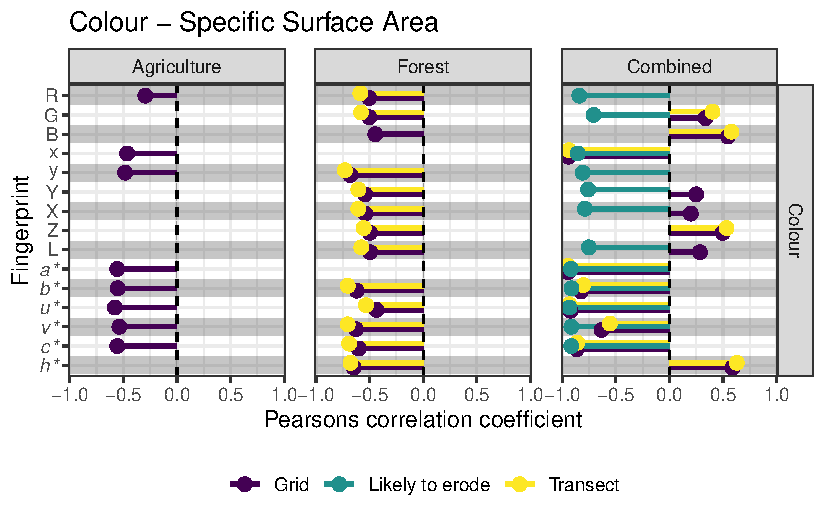
\includegraphics{index_files/figure-pdf/unnamed-chunk-2-1.pdf}

\textsubscript{Source:
\href{https://alex-koiter.github.io/sampling-design-manuscript/index.qmd.html}{Article
Notebook}}

}

\caption{\label{suppplot-supfig1}Pearsons correlation coefficients for
colour properties and specific surface area for each site independently
and both sites combined. Fingerprints that did not have a significant
correlation (p value \textless{} 0.05) were omitted.}

\end{suppplot}%

\begin{suppplot}

\centering{

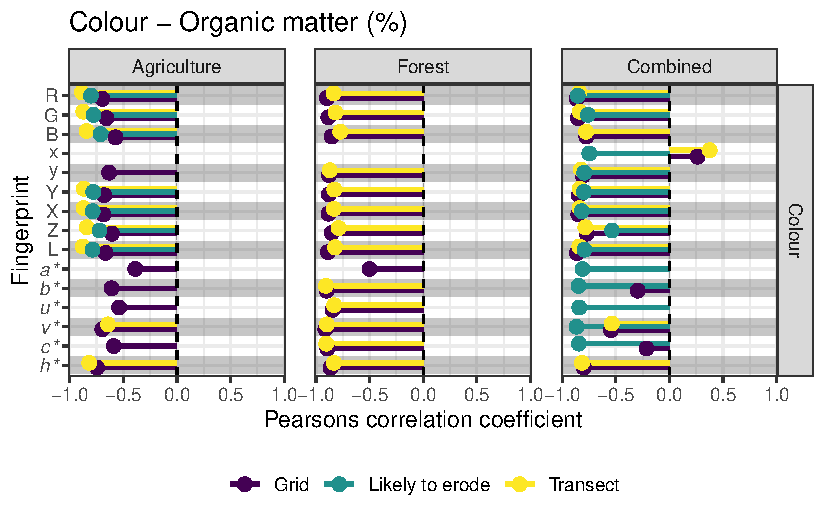
\includegraphics{index_files/figure-pdf/unnamed-chunk-3-1.pdf}

\textsubscript{Source:
\href{https://alex-koiter.github.io/sampling-design-manuscript/index.qmd.html}{Article
Notebook}}

}

\caption{\label{suppplot-supfig2}Pearsons correlation coefficients for
colour properties and soil organic matter content for each site
independently and both sites combined. Fingerprints that did not have a
significant correlation (p value \textless{} 0.05) were omitted.}

\end{suppplot}%

\begin{suppplot}

\centering{

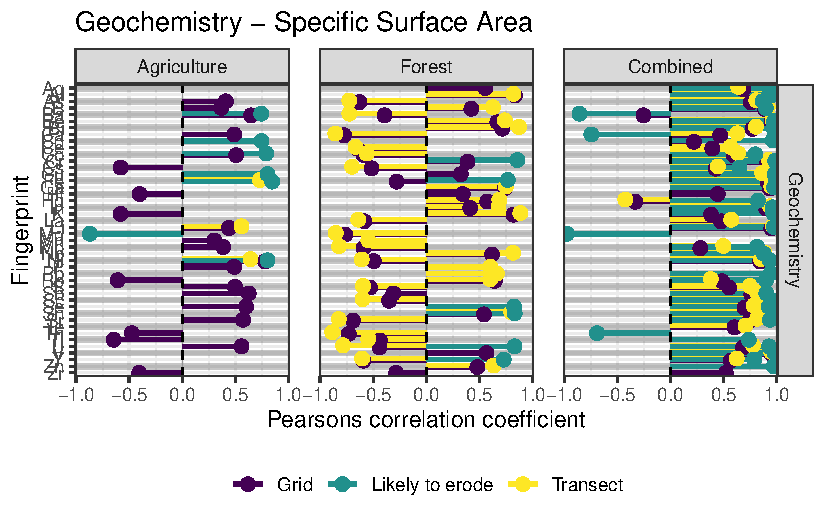
\includegraphics{index_files/figure-pdf/unnamed-chunk-4-1.pdf}

\textsubscript{Source:
\href{https://alex-koiter.github.io/sampling-design-manuscript/index.qmd.html}{Article
Notebook}}

}

\caption{\label{suppplot-supfig3}Pearsons correlation coefficients for
colour properties and specific surface area for each site independently
and both sites combined. Fingerprints that did not have a significant
correlation (p value \textless{} 0.05) were omitted.}

\end{suppplot}%

\begin{suppplot}

\centering{

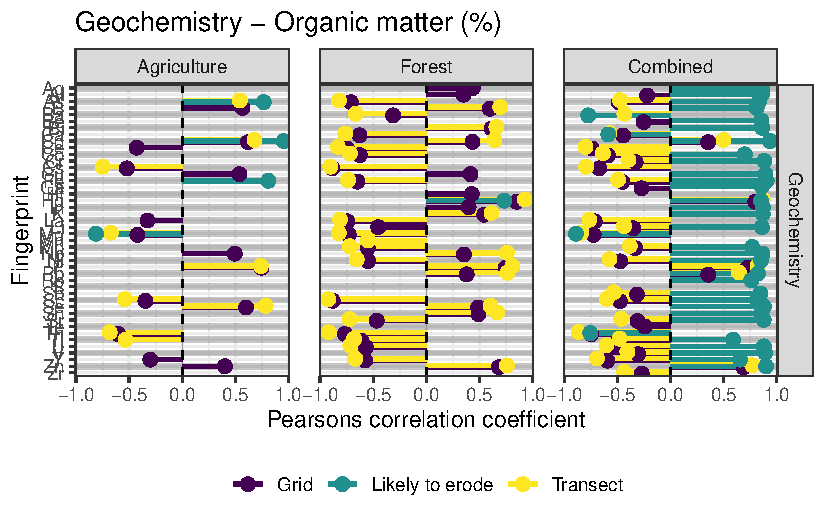
\includegraphics{index_files/figure-pdf/unnamed-chunk-5-1.pdf}

\textsubscript{Source:
\href{https://alex-koiter.github.io/sampling-design-manuscript/index.qmd.html}{Article
Notebook}}

}

\caption{\label{suppplot-supfig4}Pearsons correlation coefficients for
colour properties and soil organic matter content for each site
independently and both sites combined. Fingerprints that did not have a
significant correlation (p value \textless{} 0.05) were omitted.}

\end{suppplot}%

\begin{suppplot}

\centering{

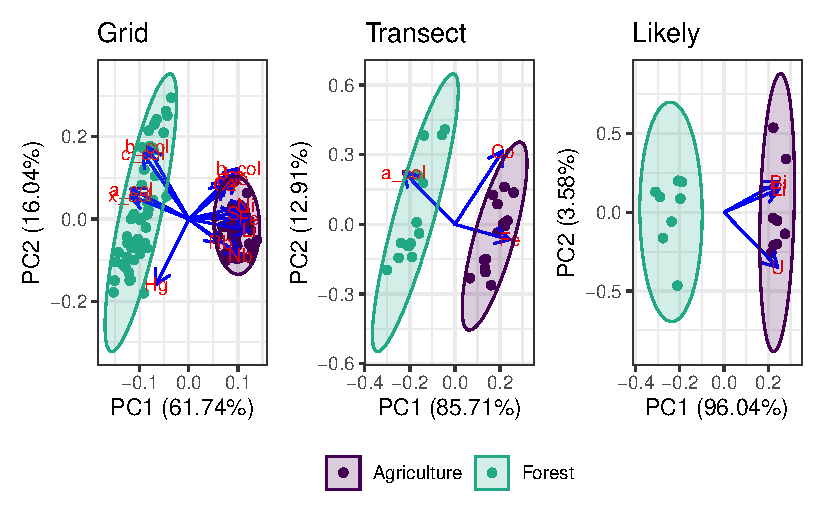
\includegraphics{index_files/figure-pdf/unnamed-chunk-6-1.pdf}

\textsubscript{Source:
\href{https://alex-koiter.github.io/sampling-design-manuscript/index.qmd.html}{Article
Notebook}}

}

\caption{\label{suppplot-supfig5}Principle component analysis and
loadings demonstrating the discriminatory ability for the selected
fingerprints for the three sampling designs.}

\end{suppplot}%

\begin{suppplot}

\centering{

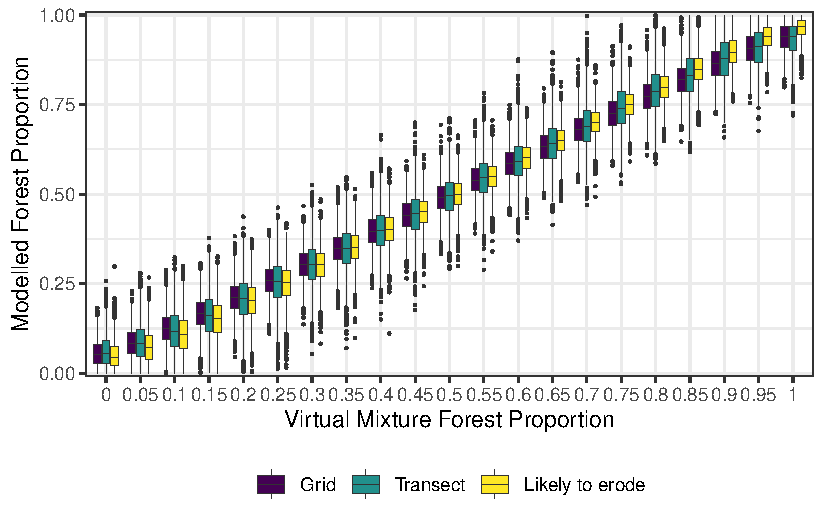
\includegraphics{index_files/figure-pdf/unnamed-chunk-7-1.pdf}

\textsubscript{Source:
\href{https://alex-koiter.github.io/sampling-design-manuscript/index.qmd.html}{Article
Notebook}}

}

\caption{\label{suppplot-supfig6}Comparison of the posterior
distribution of the modeled proportion of forest source to the
proportion of forest source in the virtual mixtures for each of the
three sampling designs using the design specific mixtures.}

\end{suppplot}%

\begin{suppplot}

\centering{

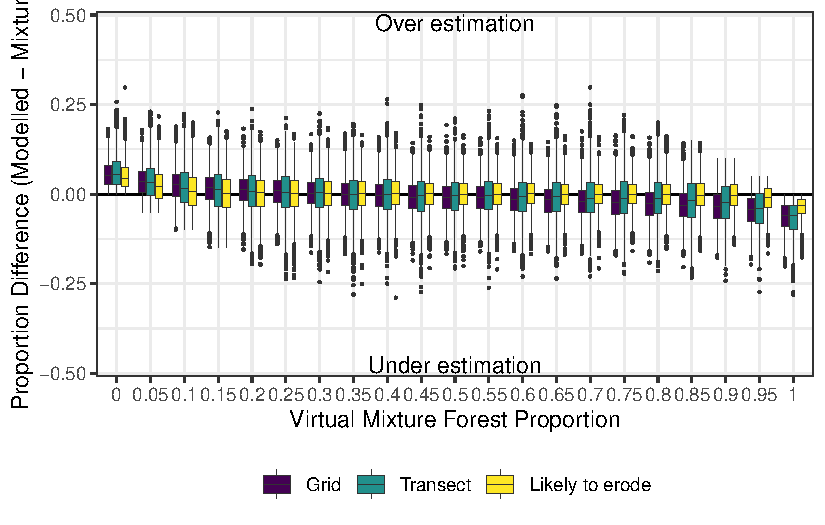
\includegraphics{index_files/figure-pdf/unnamed-chunk-8-1.pdf}

\textsubscript{Source:
\href{https://alex-koiter.github.io/sampling-design-manuscript/index.qmd.html}{Article
Notebook}}

}

\caption{\label{suppplot-supfig7}Differences in the proportions between
modeled and virtual design specific mixtures.}

\end{suppplot}%

\begin{suppplot}

\centering{

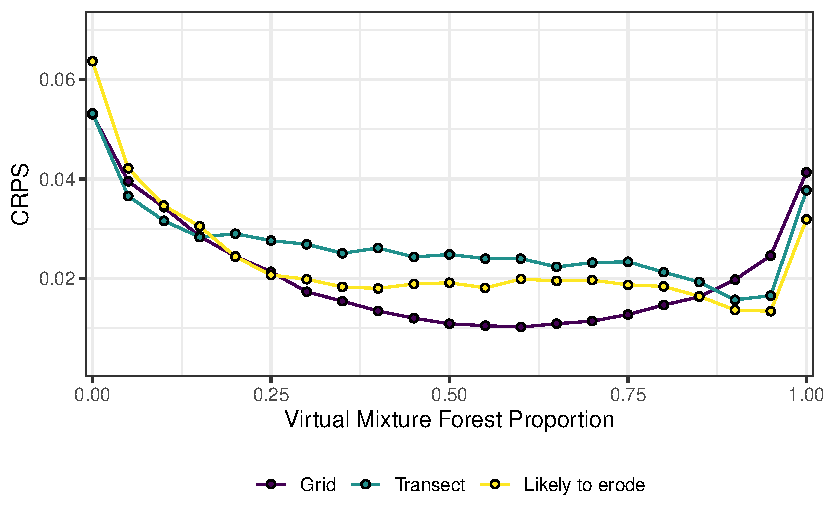
\includegraphics{index_files/figure-pdf/unnamed-chunk-9-1.pdf}

\textsubscript{Source:
\href{https://alex-koiter.github.io/sampling-design-manuscript/index.qmd.html}{Article
Notebook}}

}

\caption{\label{suppplot-supfig8}Relation between virtual mixture source
proportions and the CRPS for the three different sampling designs.}

\end{suppplot}%

\begin{suppplot}

\centering{

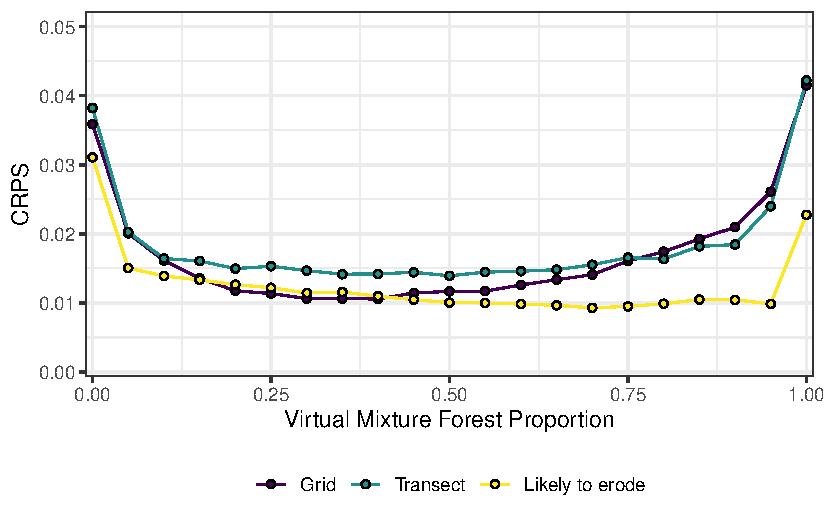
\includegraphics{index_files/figure-pdf/unnamed-chunk-10-1.pdf}

\textsubscript{Source:
\href{https://alex-koiter.github.io/sampling-design-manuscript/index.qmd.html}{Article
Notebook}}

}

\caption{\label{suppplot-supfig9}Relation between virtual mixture source
proportions and the CRPS for the three different sampling designs using
the design specific mixtures.}

\end{suppplot}%

\section*{Supplemental tables}\label{supplemental-tables}
\addcontentsline{toc}{section}{Supplemental tables}

\begin{supptab}

\caption{\label{supptab-colour-abbrev}Description of spectral
reflectance colour coefficients used as fingerprints. Reproduced from
Boudreault et al.~(2018)}

\centering{

\begin{longtable*}{ll}
\toprule
Parameter & Abbreviation \\ 
\midrule
\multicolumn{2}{l}{RGB} \\ 
\midrule
Red & R \\ 
Green & G \\ 
Blue & B \\ 
\midrule
\multicolumn{2}{l}{CIE xyY} \\ 
\midrule
Chromatic coordinate x & x \\ 
Chromatic coordinate y & y \\ 
Brightness & Y \\ 
\midrule
\multicolumn{2}{l}{CIE LAB} \\ 
\midrule
Metric lightness function & L \\ 
Chromatic coordinate opponent red–green scales & a* \\ 
Chromatic coordinate opponent blue–yellow scales & b* \\ 
\midrule
\multicolumn{2}{l}{CIE LUV} \\ 
\midrule
Chromatic coordinate opponent red–green scales & u* \\ 
Chromatic coordinate opponent blue–yellow scales & v* \\ 
\midrule
\multicolumn{2}{l}{CIE LCH} \\ 
\midrule
CIE hue & c* \\ 
CIE chroma & h* \\ 
\bottomrule
\end{longtable*}

\textsubscript{Source:
\href{https://alex-koiter.github.io/sampling-design-manuscript/index.qmd.html}{Article
Notebook}}

}

\end{supptab}%

\begin{supptab}

\caption{\label{supptab-model-eq}Model evaluation metric and criteria}

\centering{

\begin{longtable*}[]{@{}
  >{\raggedright\arraybackslash}p{(\columnwidth - 6\tabcolsep) * \real{0.2466}}
  >{\raggedright\arraybackslash}p{(\columnwidth - 6\tabcolsep) * \real{0.2466}}
  >{\raggedright\arraybackslash}p{(\columnwidth - 6\tabcolsep) * \real{0.2603}}
  >{\raggedright\arraybackslash}p{(\columnwidth - 6\tabcolsep) * \real{0.2466}}@{}}
\toprule\noalign{}
\begin{minipage}[b]{\linewidth}\raggedright
Criteria
\end{minipage} & \begin{minipage}[b]{\linewidth}\raggedright
Parameter
\end{minipage} & \begin{minipage}[b]{\linewidth}\raggedright
Equation
\end{minipage} & \begin{minipage}[b]{\linewidth}\raggedright
Reference
\end{minipage} \\
\midrule\noalign{}
\endhead
\bottomrule\noalign{}
\endlastfoot
Uncertainty & Interval accuracy (P) &
\(                                                                                                                                                                                                                                                                                                                                                                                                                                                                                                                                                                                                                                                                                                                                                                                                                                                                                                                                                                                                                                                                                                                                                                                                                                                                                                                                                                                                                                                                                                                                                                                                                                                                                                                                                                                                                                                                                                                                                                                                                                                                                                                                                                                                                                                                                                                             
                                                                                                                                                                                                                                                                                                                                                                                                                                                                                                                                                                                                                                                                                                                                                                                                                                                                                                                                                                                                                                                                                                                                                                                                                                                                                                                                                                                                                                                                                                                                                                                                                                                                                                                                                                                                                                                                                                                                                                                                                                                                                                                                                                                                                                                                        \frac{encompassed} {total}                                                                                               
                                                                                                                                                                                                                                                                                                                                                                                                                                                                                                                                                                                                                                                                                                                                                                                                                                                                                                                                                                                                                                                                                                                                                                                                                                                                                                                                                                                                                                                                                                                                                                                                                                                                                                                                                                                                                                                                                                                                                                                                                                                                                                                                                                                                                                                                        \)
& \\
Uncertainty & Interval width (W) &
\(                                                                                                                                                                                                                                                                                                                                                                                                                                                                                                                                                                                                                                                                                                                                                                                                                                                                                                                                                                                                                                                                                                                                                                                                                                                                                                                                                                                                                                                                                                                                                                                                                                                                                                                                                                                                                                                                                                                                                                                                                                                                                                                                                                                                                                                                                                                             
                                                                                                                                                                                                                                                                                                                                                                                                                                                                                                                                                                                                                                                                                                                                                                                                                                                                                                                                                                                                                                                                                                                                                                                                                                                                                                                                                                                                                                                                                                                                                                                                                                                                                                                                                                                                                                                                                                                                                                                                                                                                                                                                                                                                                                                                        upperquantile − lowerquantile                                                                                            
                                                                                                                                                                                                                                                                                                                                                                                                                                                                                                                                                                                                                                                                                                                                                                                                                                                                                                                                                                                                                                                                                                                                                                                                                                                                                                                                                                                                                                                                                                                                                                                                                                                                                                                                                                                                                                                                                                                                                                                                                                                                                                                                                                                                                                                                        \)
& \\
Residual methods & Mean absolute error (MAE) &
\(                                                                                                                                                                                                                                                                                                                                                                                                                                                                                                                                                                                                                                                                                                                                                                                                                                                                                                                                                                                                                                                                                                                                                                                                                                                                                                                                                                                                                                                                                                                                                                                                                                                                                                                                                                                                                                                                                                                                                                                                                                                                                                                                                                                                                                                                                                                             
                                                                                                                                                                                                                                                                                                                                                                                                                                                                                                                                                                                                                                                                                                                                                                                                                                                                                                                                                                                                                                                                                                                                                                                                                                                                                                                                                                                                                                                                                                                                                                                                                                                                                                                                                                                                                                                                                                                                                                                                                                                                                                                                                                                                                                 \frac{1}{n}\sum_{i=1}^{n} |y_i -\hat{y_i}|                                                                                                                      
                                                                                                                                                                                                                                                                                                                                                                                                                                                                                                                                                                                                                                                                                                                                                                                                                                                                                                                                                                                                                                                                                                                                                                                                                                                                                                                                                                                                                                                                                                                                                                                                                                                                                                                                                                                                                                                                                                                                                                                                                                                                                                                                                                                                                                 \)
& Bennett et al.~(2013) \\
Residual methods & Mean error (ME) &
\(                                                                                                                                                                                                                                                                                                                                                                                                                                                                                                                                                                                                                                                                                                                                                                                                                                                                                                                                                                                                                                                                                                                                                                                                                                                                                                                                                                                                                                                                                                                                                                                                                                                                                                                                                                                                                                                                                                                                                                                                                                                                                                                                                                                                                                                                                                                             
                                                                                                                                                                                                                                                                                                                                                                                                                                                                                                                                                                                                                                                                                                                                                                                                                                                                                                                                                                                                                                                                                                                                                                                                                                                                                                                                                                                                                                                                                                                                                                                                                                                                                                                                                                                                                                                                                                                                                                                                                                                                                                                                                                                                                                 \frac{1}{n}\sum_{i=1}^{n} (y_i -\hat{y_i})                                                                                                                      
                                                                                                                                                                                                                                                                                                                                                                                                                                                                                                                                                                                                                                                                                                                                                                                                                                                                                                                                                                                                                                                                                                                                                                                                                                                                                                                                                                                                                                                                                                                                                                                                                                                                                                                                                                                                                                                                                                                                                                                                                                                                                                                                                                                                                                 \)
& Bennett et al.~(2013) \\
Performance & Continuous ranked probability score (CRPS) &
\(                                                                                                                                                                                                                                                                                                                                                                                                                                                                                                                                                                                                                                                                                                                                                                                                                                                                                                                                                                                                                                                                                                                                                                                                                                                                                                                                                                                                                                                                                                                                                                                                                                                                                                                                                                                                                                                                                                                                                                                                                                                                                                                                                                                                                                                                                                                             
                                                                                                                                                                                                                                                                                                                                                                                                                                                                                                                                                                                                                                                                                                                                                                                                                                                                                                                                                                                                                                                                                                                                                                                                                                                                                                                                                                                                                                                                                                                                                                                                                                                                                                                                                                                                                                                                                                                                                                                                                                                                                                                                                                                                                                 (F_i,y_i) = \int_{-\infty}^\infty (F_i(y_i)-H[y_i \geq \hat{y}]^2 dx                                                                                            
                                                                                                                                                                                                                                                                                                                                                                                                                                                                                                                                                                                                                                                                                                                                                                                                                                                                                                                                                                                                                                                                                                                                                                                                                                                                                                                                                                                                                                                                                                                                                                                                                                                                                                                                                                                                                                                                                                                                                                                                                                                                                                                                                                                                                                 \)
& Matheson and Winkler (1976) \\
Performance & Nash--Sutcliffe efficiency index (NSE) &
\(                                                                                                                                                                                                                                                                                                                                                                                                                                                                                                                                                                                                                                                                                                                                                                                                                                                                                                                                                                                                                                                                                                                                                                                                                                                                                                                                                                                                                                                                                                                                                                                                                                                                                                                                                                                                                                                                                                                                                                                                                                                                                                                                                                                                                                                                                                                             
                                                                                                                                                                                                                                                                                                                                                                                                                                                                                                                                                                                                                                                                                                                                                                                                                                                                                                                                                                                                                                                                                                                                                                                                                                                                                                                                                                                                                                                                                                                                                                                                                                                                                                                                                                                                                                                                                                                                                                                                                                                                                                                                                                                                                                 1-\frac{\frac{1}{n}\sum_{1}^{n}(yi - \hat{y_i})^2} {\frac{1}{n}\sum_{1}^{n}(yi - \bar{y_i})^2}                                                                  
                                                                                                                                                                                                                                                                                                                                                                                                                                                                                                                                                                                                                                                                                                                                                                                                                                                                                                                                                                                                                                                                                                                                                                                                                                                                                                                                                                                                                                                                                                                                                                                                                                                                                                                                                                                                                                                                                                                                                                                                                                                                                                                                                                                                                                 \)
& Nash and Sutcliffe (1970) \\
Contingency & Critical success index (CSI) &
\(                                                                                                                                                                                                                                                                                                                                                                                                                                                                                                                                                                                                                                                                                                                                                                                                                                                                                                                                                                                                                                                                                                                                                                                                                                                                                                                                                                                                                                                                                                                                                                                                                                                                                                                                                                                                                                                                                                                                                                                                                                                                                                                                                                                                                                                                                                                             
                                                                                                                                                                                                                                                                                                                                                                                                                                                                                                                                                                                                                                                                                                                                                                                                                                                                                                                                                                                                                                                                                                                                                                                                                                                                                                                                                                                                                                                                                                                                                                                                                                                                                                                                                                                                                                                                                                                                                                                                                                                                                                                                                                                                                                 \frac{hits}{hits+misses+falsealarms}                                                                                                                            
                                                                                                                                                                                                                                                                                                                                                                                                                                                                                                                                                                                                                                                                                                                                                                                                                                                                                                                                                                                                                                                                                                                                                                                                                                                                                                                                                                                                                                                                                                                                                                                                                                                                                                                                                                                                                                                                                                                                                                                                                                                                                                                                                                                                                                 \)
& Bennett et al.~(2013) \\
Contingency & Hit rate (HR) &
\(                                                                                                                                                                                                                                                                                                                                                                                                                                                                                                                                                                                                                                                                                                                                                                                                                                                                                                                                                                                                                                                                                                                                                                                                                                                                                                                                                                                                                                                                                                                                                                                                                                                                                                                                                                                                                                                                                                                                                                                                                                                                                                                                                                                                                                                                                                                             
                                                                                                                                                                                                                                                                                                                                                                                                                                                                                                                                                                                                                                                                                                                                                                                                                                                                                                                                                                                                                                                                                                                                                                                                                                                                                                                                                                                                                                                                                                                                                                                                                                                                                                                                                                                                                                                                                                                                                                                                                                                                                                                                                                                                                                 \frac{hits}{hits+misses}                                                                                                                                        
                                                                                                                                                                                                                                                                                                                                                                                                                                                                                                                                                                                                                                                                                                                                                                                                                                                                                                                                                                                                                                                                                                                                                                                                                                                                                                                                                                                                                                                                                                                                                                                                                                                                                                                                                                                                                                                                                                                                                                                                                                                                                                                                                                                                                                 \)
& Bennett et al.~(2013) \\
& & & \\
\end{longtable*}

}

\end{supptab}%

\begin{supptab}

\caption{\label{supptab-corr-summary}Overall summary of significant (p
\textless0.05) Pearsons correlations between soil properties, specific
surface area (SSA) and organic matter content, and fingerprinting
properties.}

\centering{

\begin{longtable*}{lclrrr}
\toprule
Site & Property & Fingerprint & No. fingerprints & No. p < 0.05 & \% p<0.05 \\ 
\midrule
\multicolumn{6}{l}{Grid} \\ 
\midrule
Agriculture & Organic matter & Colour & 15 & 14 & $93.3$ \\ 
Agriculture & Organic matter & Geochemistry & 44 & 14 & $31.8$ \\ 
Agriculture & SSA & Colour & 15 & 8 & $53.3$ \\ 
Agriculture & SSA & Geochemistry & 44 & 22 & $50.0$ \\ 
Combined & Organic matter & Colour & 15 & 13 & $86.7$ \\ 
Combined & Organic matter & Geochemistry & 44 & 30 & $68.2$ \\ 
Combined & SSA & Colour & 15 & 13 & $86.7$ \\ 
Combined & SSA & Geochemistry & 44 & 37 & $84.1$ \\ 
Forest & Organic matter & Colour & 15 & 14 & $93.3$ \\ 
Forest & Organic matter & Geochemistry & 44 & 34 & $77.3$ \\ 
Forest & SSA & Colour & 15 & 13 & $86.7$ \\ 
Forest & SSA & Geochemistry & 44 & 37 & $84.1$ \\ 
\midrule
\multicolumn{6}{l}{Likely to erode} \\ 
\midrule
Agriculture & Organic matter & Colour & 15 & 7 & $46.7$ \\ 
Agriculture & Organic matter & Geochemistry & 44 & 4 & $9.1$ \\ 
Agriculture & SSA & Colour & 15 & 0 & $0.0$ \\ 
Agriculture & SSA & Geochemistry & 44 & 7 & $15.9$ \\ 
Combined & Organic matter & Colour & 15 & 13 & $86.7$ \\ 
Combined & Organic matter & Geochemistry & 44 & 35 & $79.5$ \\ 
Combined & SSA & Colour & 15 & 12 & $80.0$ \\ 
Combined & SSA & Geochemistry & 44 & 36 & $81.8$ \\ 
Forest & Organic matter & Colour & 15 & 0 & $0.0$ \\ 
Forest & Organic matter & Geochemistry & 44 & 1 & $2.3$ \\ 
Forest & SSA & Colour & 15 & 0 & $0.0$ \\ 
Forest & SSA & Geochemistry & 44 & 6 & $13.6$ \\ 
\midrule
\multicolumn{6}{l}{Transect} \\ 
\midrule
Agriculture & Organic matter & Colour & 15 & 9 & $60.0$ \\ 
Agriculture & Organic matter & Geochemistry & 44 & 9 & $20.5$ \\ 
Agriculture & SSA & Colour & 15 & 0 & $0.0$ \\ 
Agriculture & SSA & Geochemistry & 44 & 3 & $6.8$ \\ 
Combined & Organic matter & Colour & 15 & 11 & $73.3$ \\ 
Combined & Organic matter & Geochemistry & 44 & 27 & $61.4$ \\ 
Combined & SSA & Colour & 15 & 10 & $66.7$ \\ 
Combined & SSA & Geochemistry & 44 & 32 & $72.7$ \\ 
Forest & Organic matter & Colour & 15 & 13 & $86.7$ \\ 
Forest & Organic matter & Geochemistry & 44 & 29 & $65.9$ \\ 
Forest & SSA & Colour & 15 & 12 & $80.0$ \\ 
Forest & SSA & Geochemistry & 44 & 32 & $72.7$ \\ 
\bottomrule
\end{longtable*}

\textsubscript{Source:
\href{https://alex-koiter.github.io/sampling-design-manuscript/index.qmd.html}{Article
Notebook}}

}

\end{supptab}%

\begin{supptab}

\caption{\label{supptab-range-test}Fingerprint properties that passed
the range test for conservative behavior for each sampling approach
using the design specific mixtures.}

\centering{

\begin{longtable*}[]{@{}
  >{\raggedright\arraybackslash}p{(\columnwidth - 2\tabcolsep) * \real{0.3472}}
  >{\raggedright\arraybackslash}p{(\columnwidth - 2\tabcolsep) * \real{0.6528}}@{}}
\toprule\noalign{}
\begin{minipage}[b]{\linewidth}\raggedright
Sampling design
\end{minipage} & \begin{minipage}[b]{\linewidth}\raggedright
Fingerprinting properties
\end{minipage} \\
\midrule\noalign{}
\endhead
\bottomrule\noalign{}
\endlastfoot
Grid & Ag Al As Ba Be Bi Ca Cd Ce Co Cr Cs Cu Fe Ga Hf Hg In K La Li Mg
Mn Mo Nb Ni P Pb Rb S Sb Sc Se Sn Sr Te Th Tl U V Y Zn Zr \emph{R G B x*
y* Y X Z L a* b* u* v* c* h*} \\
Transect & Ag Al As B Ba Be Bi Ca Cd Ce Co Cr Cs Cu Fe Ga Hf Hg In K La
Li Mg Mn Mo Nb Ni P Pb Rb S Sb Sc Se Sn Sr Te Th Tl U V Y Zn Zr \emph{R
G B x* y* Y X Z L a* b* u* v* c* h*} \\
Likely to erode & Ag Al As B Ba Be Bi Ca Cd Ce Co Cr Cs Cu Fe Ga Hf Hg
In K La Li Mg Mn Mo Nb Ni P Pb Rb S Sb Sc Se Sn Sr Te Th Tl U V Y Zn Zr
\emph{R G B x* y* Y X Z L a* b* u* v* c* h*} \\
\end{longtable*}

}

\end{supptab}%

\begin{supptab}

\caption{\label{supptab-KW-test}Fingerprint properties that passed the
Mann Whitney test for each sampling approach using the design specific
mixtures.}

\centering{

\begin{longtable*}[]{@{}
  >{\raggedright\arraybackslash}p{(\columnwidth - 2\tabcolsep) * \real{0.3472}}
  >{\raggedright\arraybackslash}p{(\columnwidth - 2\tabcolsep) * \real{0.6528}}@{}}
\toprule\noalign{}
\begin{minipage}[b]{\linewidth}\raggedright
Sampling design
\end{minipage} & \begin{minipage}[b]{\linewidth}\raggedright
Fingerprinting properties
\end{minipage} \\
\midrule\noalign{}
\endhead
\bottomrule\noalign{}
\endlastfoot
Grid & Ag Al As Be Bi Ca Cd Ce Co Cr Cs Cu Fe Ga Hf Hg In K La Li Mg Nb
Ni Rb S Sb Sc Se Sn Sr Te Th U V Y Zr \emph{G B x Y X Z L a* b* u* v* c*
h*} \\
Transect & Ag Al As B Be Bi Ca Cd Ce Co Cr Cs Cu Fe Ga In La Li Nb Ni S
Sb Sc Se Sn Sr Te U V Y \emph{B x* Z a* b* u* c* h*} \\
Likely to erode & Ag Al As B Ba Be Bi Ca Cd Co Cr Cs Cu Fe Ga Hg In K Li
Mg Mo Nb Ni Pb Rb Sb Sc Se Sn Sr Th Tl U V Y Zn \emph{R G x* y* Y X L a*
b* u* v* c*} \\
\end{longtable*}

}

\end{supptab}%

\begin{supptab}

\caption{\label{supptab-DFA}Results of the stepwise DFA for each
sampling approach including the percent of samples correctly classified
for each site using the design specific mixtures.}

\begin{minipage}{\linewidth}

\begin{longtable}[]{@{}
  >{\raggedright\arraybackslash}p{(\columnwidth - 6\tabcolsep) * \real{0.7000}}
  >{\raggedright\arraybackslash}p{(\columnwidth - 6\tabcolsep) * \real{0.1000}}
  >{\raggedright\arraybackslash}p{(\columnwidth - 6\tabcolsep) * \real{0.1000}}
  >{\raggedright\arraybackslash}p{(\columnwidth - 6\tabcolsep) * \real{0.1000}}@{}}
\caption{Grid sampling design}\tabularnewline
\toprule\noalign{}
\begin{minipage}[b]{\linewidth}\raggedright
Composite fingerprint
\end{minipage} & \begin{minipage}[b]{\linewidth}\raggedright
Wilks' lambda
\end{minipage} & \begin{minipage}[b]{\linewidth}\raggedright
Agriculture
\end{minipage} & \begin{minipage}[b]{\linewidth}\raggedright
Forest
\end{minipage} \\
\midrule\noalign{}
\endfirsthead
\toprule\noalign{}
\begin{minipage}[b]{\linewidth}\raggedright
Composite fingerprint
\end{minipage} & \begin{minipage}[b]{\linewidth}\raggedright
Wilks' lambda
\end{minipage} & \begin{minipage}[b]{\linewidth}\raggedright
Agriculture
\end{minipage} & \begin{minipage}[b]{\linewidth}\raggedright
Forest
\end{minipage} \\
\midrule\noalign{}
\endhead
\bottomrule\noalign{}
\endlastfoot
Li & 0.062 & 100 & 100 \\
Li + \emph{a*} & 0.044 & 100 & 100 \\
Li + \emph{a*} + Fe & 0.028 & 100 & 100 \\
Li + \emph{a*} + Fe + Co & 0.023 & 100 & 100 \\
Li + \emph{a*} + Fe + Co + Hg & 0.022 & 100 & 100 \\
Li + \emph{a*} + Fe + Co + Hg + \emph{x*} & 0.019 & 100 & 100 \\
Li + \emph{a*} + Fe + Co + Hg + \emph{x*} + Cs & 0.018 & 100 & 100 \\
Li + \emph{a*} + Fe + Co + Hg + \emph{x*} + Cs + La & 0.015 & 100 &
100 \\
Li + \emph{a*} + Fe + Co + Hg + \emph{x*} + Cs + La + Ni & 0.013 & 100 &
100 \\
Li + \emph{a*} + Fe + Co + Hg + \emph{x*} + Cs + La + Ni + Nb & 0.013 &
100 & 100 \\
Li + \emph{a*} + Fe + Co + Hg + \emph{x*} + Cs + La + Ni + Nb +
\emph{h*} & 0.012 & 100 & 100 \\
Li + \emph{a*} + Fe + Co + Hg + \emph{x*} + Cs + La + Ni + Nb +
\emph{h*} + \emph{b*} & 0.011 & 100 & 100 \\
Li + \emph{a*} + Fe + Co + Hg + \emph{x*} + Cs + La + Ni + Nb +
\emph{h*} + \emph{b*} + Rb & 0.011 & 100 & 100 \\
Li + \emph{a*} + Fe + Co + Hg + \emph{x*} + Cs + La + Ni + Nb +
\emph{h*} + \emph{b*} + Rb + Ca & 0.010 & 100 & 100 \\
Li + \emph{a*} + Fe + Co + Hg + \emph{x*} + Cs + La + Ni + Nb +
\emph{h*} + \emph{b*} + Rb + Ca + Sr & 0.009 & 100 & 100 \\
Li + \emph{a*} + Fe + Co + Hg + \emph{x*} + Cs + La + Ni + Nb +
\emph{h*} + \emph{b*} + Rb + Ca + Sr + \emph{c*} & 0.009 & 100 & 100 \\
\end{longtable}

\end{minipage}%
\newline
\begin{minipage}{\linewidth}

\begin{longtable}[]{@{}
  >{\raggedright\arraybackslash}p{(\columnwidth - 6\tabcolsep) * \real{0.7000}}
  >{\raggedright\arraybackslash}p{(\columnwidth - 6\tabcolsep) * \real{0.1000}}
  >{\raggedright\arraybackslash}p{(\columnwidth - 6\tabcolsep) * \real{0.1000}}
  >{\raggedright\arraybackslash}p{(\columnwidth - 6\tabcolsep) * \real{0.1000}}@{}}
\caption{Transect sampling design}\tabularnewline
\toprule\noalign{}
\begin{minipage}[b]{\linewidth}\raggedright
Composite fingerprint
\end{minipage} & \begin{minipage}[b]{\linewidth}\raggedright
Wilks' lambda
\end{minipage} & \begin{minipage}[b]{\linewidth}\raggedright
Agriculture
\end{minipage} & \begin{minipage}[b]{\linewidth}\raggedright
Forest
\end{minipage} \\
\midrule\noalign{}
\endfirsthead
\toprule\noalign{}
\begin{minipage}[b]{\linewidth}\raggedright
Composite fingerprint
\end{minipage} & \begin{minipage}[b]{\linewidth}\raggedright
Wilks' lambda
\end{minipage} & \begin{minipage}[b]{\linewidth}\raggedright
Agriculture
\end{minipage} & \begin{minipage}[b]{\linewidth}\raggedright
Forest
\end{minipage} \\
\midrule\noalign{}
\endhead
\bottomrule\noalign{}
\endlastfoot
Li & 0.048 & 100 & 100 \\
Li + Cu & 0.035 & 100 & 100 \\
Li + Cu + Ca & 0.026 & 100 & 100 \\
Li + Cu + Ca + Be & 0.021 & 100 & 100 \\
Li + Cu + Ca + Be + Co & 0.016 & 100 & 100 \\
\end{longtable}

\end{minipage}%
\newline
\begin{minipage}{\linewidth}

\begin{longtable}[]{@{}
  >{\raggedright\arraybackslash}p{(\columnwidth - 6\tabcolsep) * \real{0.7000}}
  >{\raggedright\arraybackslash}p{(\columnwidth - 6\tabcolsep) * \real{0.1000}}
  >{\raggedright\arraybackslash}p{(\columnwidth - 6\tabcolsep) * \real{0.1000}}
  >{\raggedright\arraybackslash}p{(\columnwidth - 6\tabcolsep) * \real{0.1000}}@{}}
\caption{Likely to erode sampling design}\tabularnewline
\toprule\noalign{}
\begin{minipage}[b]{\linewidth}\raggedright
Composite fingerprint
\end{minipage} & \begin{minipage}[b]{\linewidth}\raggedright
Wilks' lambda
\end{minipage} & \begin{minipage}[b]{\linewidth}\raggedright
Agriculture
\end{minipage} & \begin{minipage}[b]{\linewidth}\raggedright
Forest
\end{minipage} \\
\midrule\noalign{}
\endfirsthead
\toprule\noalign{}
\begin{minipage}[b]{\linewidth}\raggedright
Composite fingerprint
\end{minipage} & \begin{minipage}[b]{\linewidth}\raggedright
Wilks' lambda
\end{minipage} & \begin{minipage}[b]{\linewidth}\raggedright
Agriculture
\end{minipage} & \begin{minipage}[b]{\linewidth}\raggedright
Forest
\end{minipage} \\
\midrule\noalign{}
\endhead
\bottomrule\noalign{}
\endlastfoot
Li & 0.024 & 100 & 100 \\
Li + Sc & 0.008 & 100 & 100 \\
Li + Sc + Sn & 0.006 & 100 & 100 \\
\end{longtable}

\end{minipage}%

\end{supptab}%

\begin{supptab}

\caption{\label{supptab-model-performance}Model evaluation metrics
grouped by sampling design and source using the design specific
mixtures.}

\centering{

\begin{longtable*}{lrrrrrr}
\toprule
Parameter & Grid Agriculture & Grid Forest & Transect Agriculture & Transect Forest & Likely to erode Agriculture & Likely to erode Forest \\ 
\midrule
\multicolumn{7}{l}{Residuals} \\ 
\midrule
MAE50 & 0.01 & 0.01 & 0.02 & 0.02 & 0.01 & 0.01 \\ 
MAE95 & 0.00 & 0.00 & 0.00 & 0.00 & 0.00 & 0.00 \\ 
ME50 & 0.00 & 0.00 & 0.00 & 0.00 & 0.00 & 0.00 \\ 
ME95 & 0.00 & 0.00 & 0.00 & 0.00 & 0.00 & 0.00 \\ 
\midrule
\multicolumn{7}{l}{Performance} \\ 
\midrule
NSE50 & 0.99 & 0.99 & 0.99 & 0.99 & 0.99 & 0.99 \\ 
NSE95 & 1.00 & 1.00 & 1.00 & 1.00 & 1.00 & 1.00 \\ 
CRPS & 0.02 & 0.02 & 0.02 & 0.02 & 0.01 & 0.01 \\ 
\midrule
\multicolumn{7}{l}{Contingency} \\ 
\midrule
CSI50 & 0.93 & 0.92 & 0.91 & 0.91 & 0.93 & 0.93 \\ 
CSI95 & 0.82 & 0.86 & 0.81 & 0.80 & 0.87 & 0.87 \\ 
HR50 & 0.98 & 0.99 & 0.97 & 0.98 & 0.99 & 0.99 \\ 
HR95 & 1.00 & 1.00 & 1.00 & 1.00 & 1.00 & 1.00 \\ 
\midrule
\multicolumn{7}{l}{Uncertainty} \\ 
\midrule
W50 & 0.06 & 0.06 & 0.08 & 0.08 & 0.06 & 0.06 \\ 
W95 & 0.18 & 0.18 & 0.24 & 0.24 & 0.18 & 0.18 \\ 
P50 & 0.25 & 0.25 & 0.25 & 0.25 & 0.25 & 0.25 \\ 
P95 & 0.48 & 0.47 & 0.48 & 0.47 & 0.47 & 0.48 \\ 
\bottomrule
\end{longtable*}

\textsubscript{Source:
\href{https://alex-koiter.github.io/sampling-design-manuscript/index.qmd.html}{Article
Notebook}}

}

\end{supptab}%




\end{document}
